\documentclass[11pt,a4paper]{article}
\usepackage[T1]{fontenc}
\usepackage{calligra}
\usepackage{makeidx}
\usepackage{hyperref}
\usepackage{amsmath}
\usepackage{amsfonts}
\usepackage{amssymb}
\usepackage{makeidx}
\usepackage{graphicx}
\usepackage{wrapfig}
\usepackage{amsmath}
\usepackage{enumerate}
\usepackage{subfigure}
\usepackage{fancyhdr}
\usepackage{amsthm}
\usepackage{amsfonts}
\usepackage[a4paper, inner=1.5cm, outer=3cm, top=3cm, 
bottom=3cm, bindingoffset=1cm]{geometry} 

\begin{document}
\title{Numerical solution of the avvection equation using finite difference methods} 
\author{Simone Orioli} 
\date{Academic Year 2013/2014} 
\maketitle

\section{Introduction}
\emph{Given the advection equation in 1D $u_t+u_x=0$ build a numerical code to solve it on a grid with extent $x\in [0,10]$ and with initial conditions given by}
\begin{equation}\label{1.1}
u(x,t=0) = \exp [ -(x-x_0)^2]
\end{equation}
\emph{with $x_0=5$, or}
\begin{equation}\label{1.2}
u(x,t=0) = \begin{cases}
1 \text{ }\text{ if } x \in [4,6] \\
0 \text{ }\text{ otherwise}
\end{cases}
\end{equation}
\emph{Perform the time integration using the following schemes:
\begin{enumerate}
\item FTCS;
\item Lax-Friedrichs;
\item Leapfrog;
\item Lax-Wendroff.
\end{enumerate}
Use Courant factors $c_f=0.5$ and $c_f=1$ and compare the results obtained with the different methods, paying attention to their stability and dissipation properties (e.g., plot $u(x,t)$ at different times and the evolution of the L2-norm). Use at least $J=101$ points in the $x$ direction, so that the spacing $\delta x$ is at least $0.1$, and terminate your simulation at $t=20$. Use periodic boundary conditions.}
\begin{figure}[!h]
\centering
\subfigure[Plot of \eqref{1.1}]
{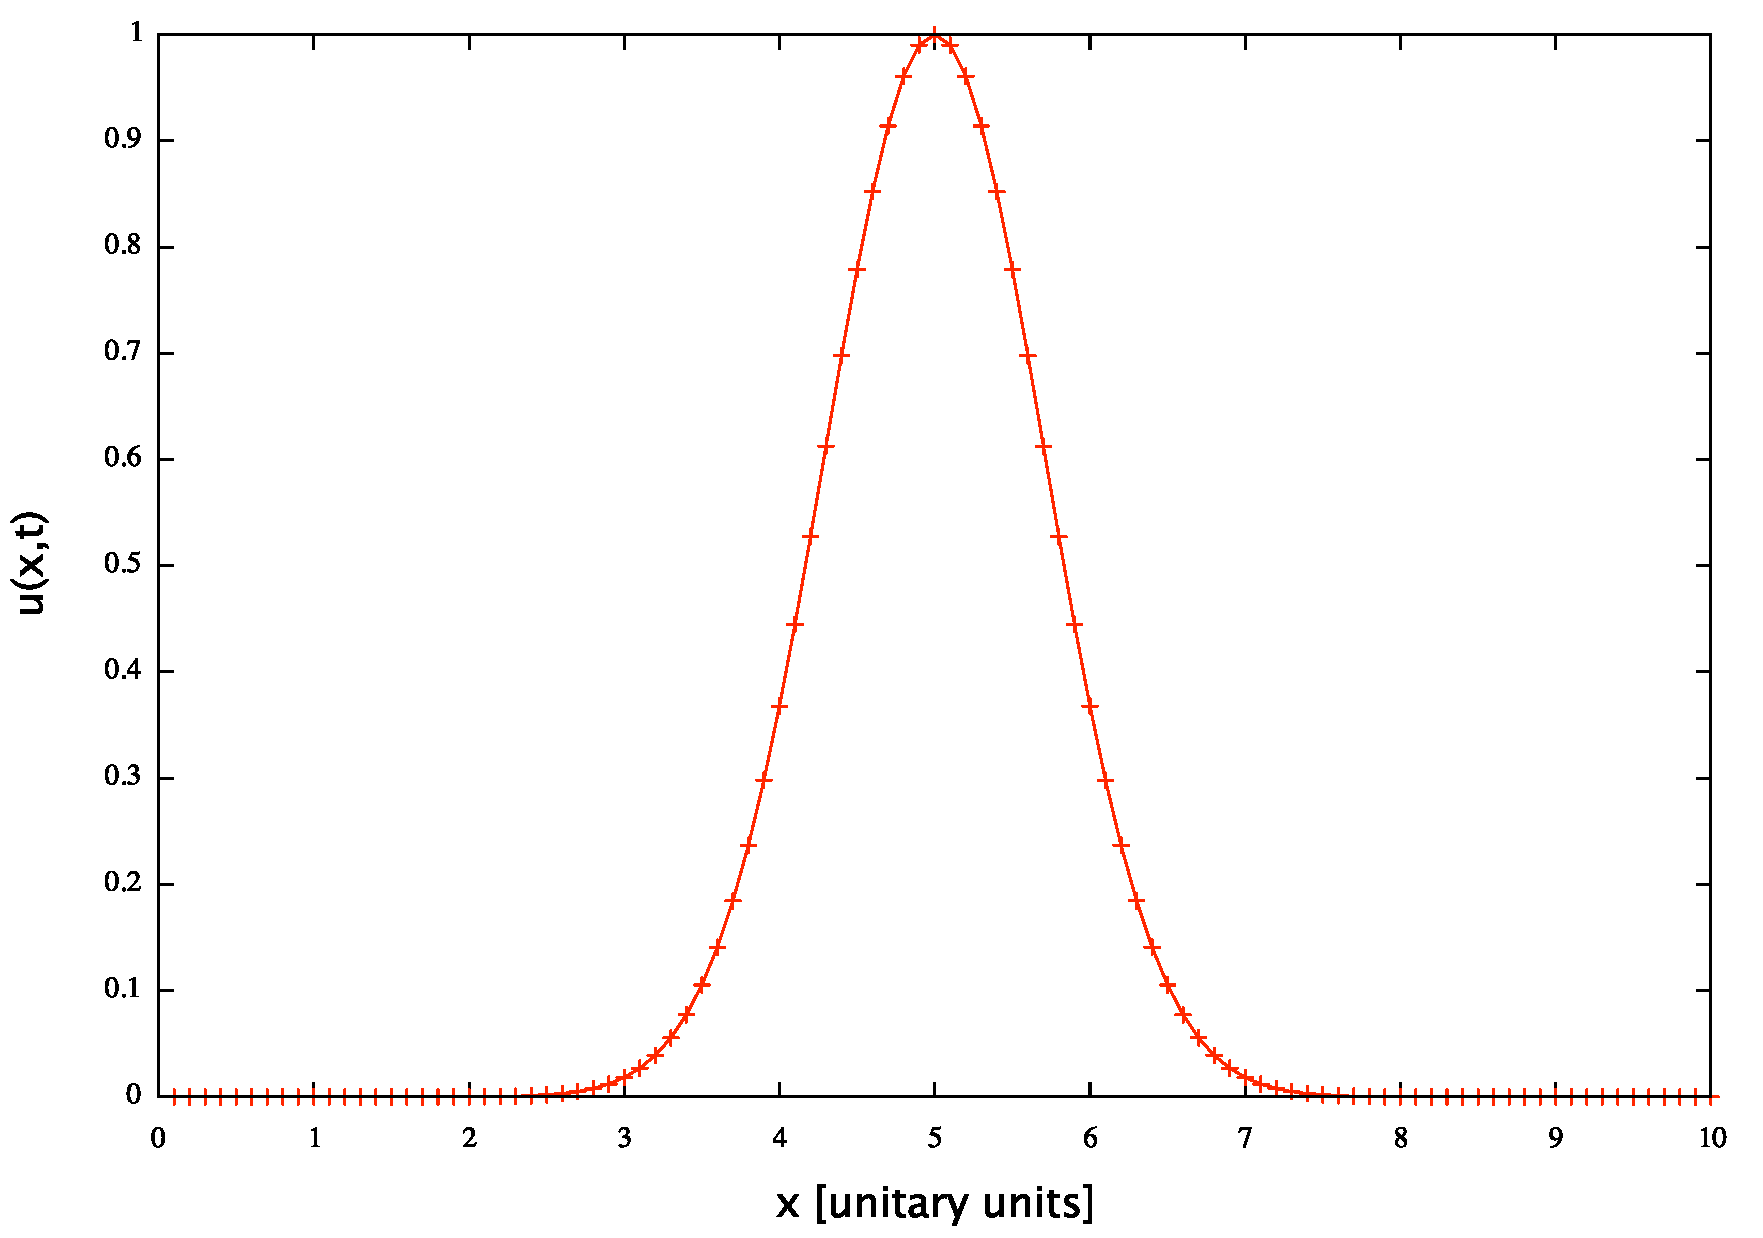
\includegraphics[scale=0.25]{gauss}}
%\hspace{5mm}
\subfigure[Plot of \eqref{1.2}]
{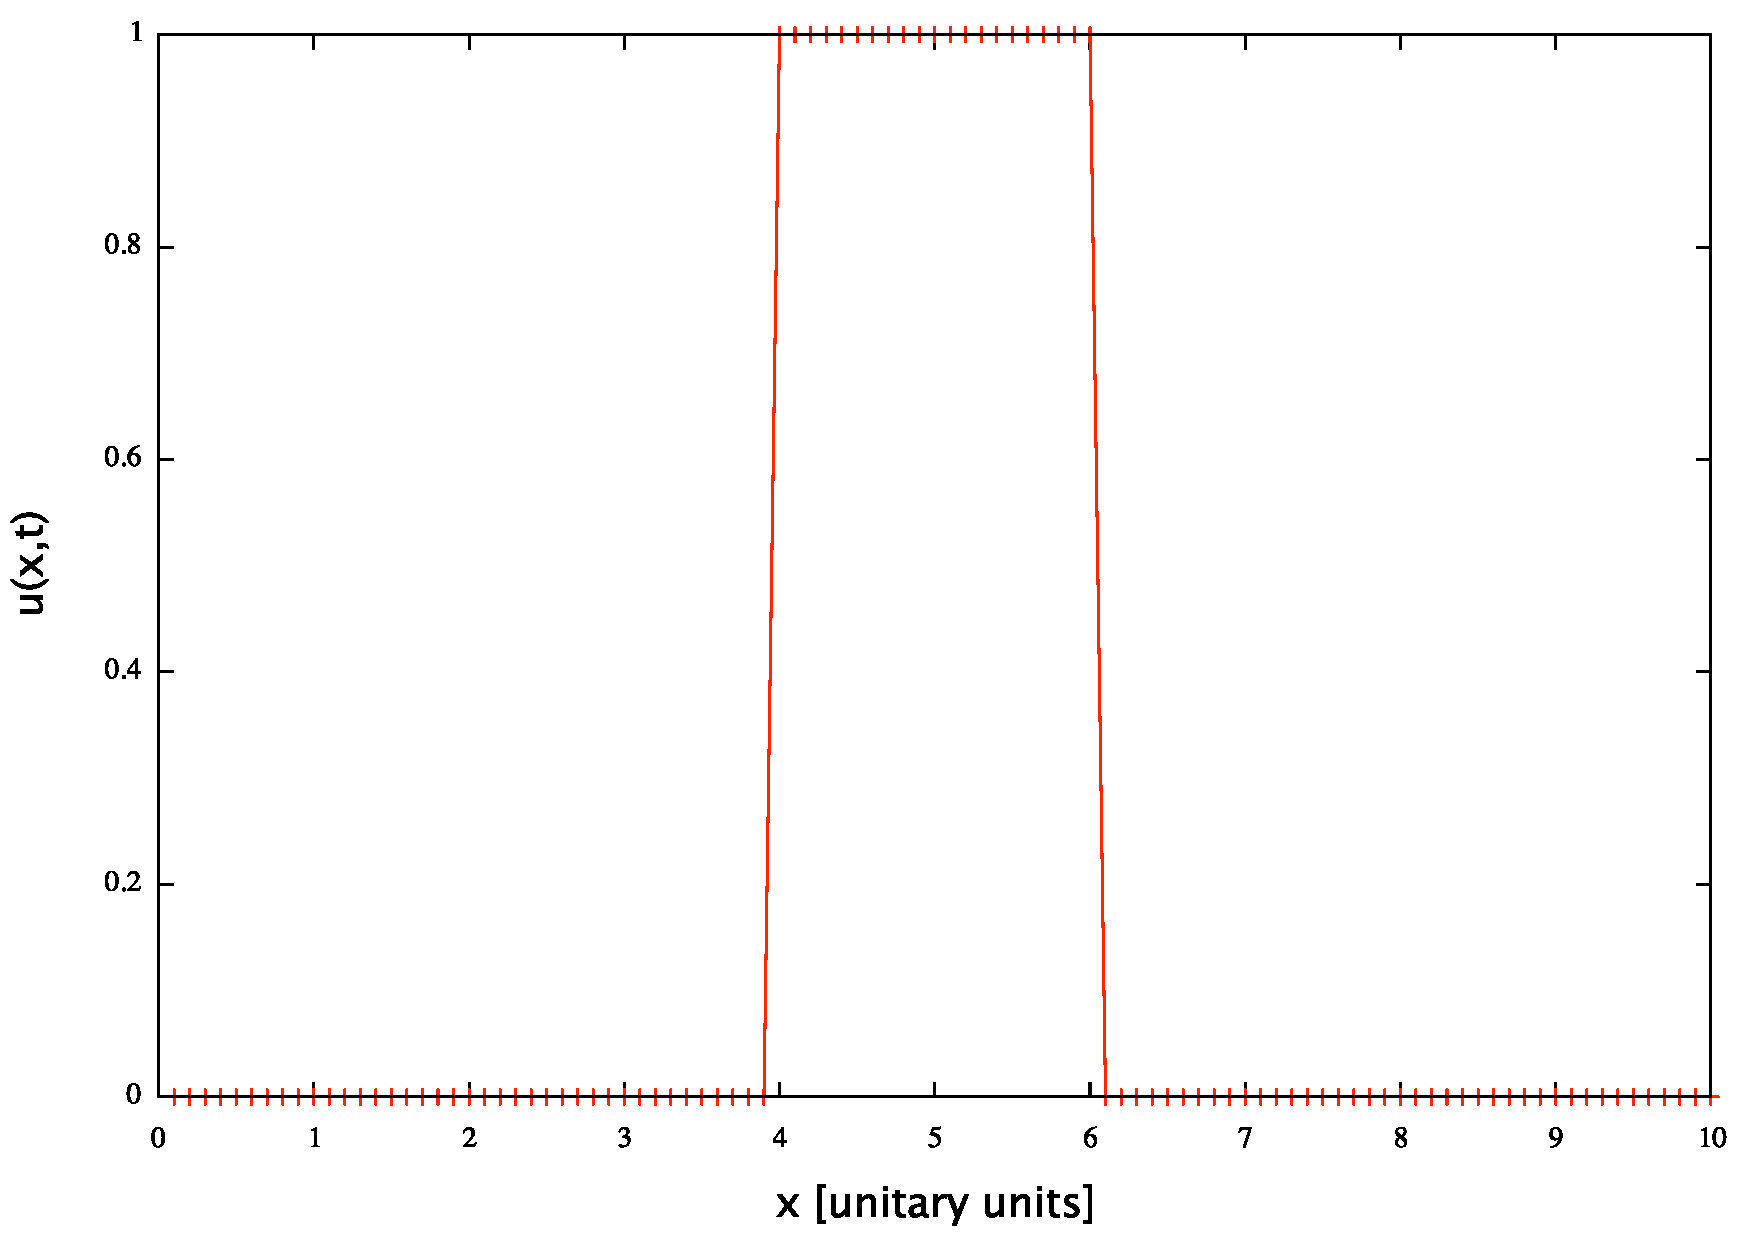
\includegraphics[scale=0.25]{sw}}
\end{figure}\ \\
We give now some basic information and definitions that will be useful in the following sections. First of all, in discussing the algorithms used to solve the avvection equation, the following notation will be used:
\begin{equation}
u_j^n \equiv u(x_j,t^n)
\end{equation}
Secondary, the peridic boundary conditions are given by the following relations:
\begin{equation}
\begin{cases}
u_0^n = u_J^n \\
u^n_{J+1}=u_1^n \\
\end{cases}
\end{equation}
while the L2-norm is the difined as
\begin{equation}
||u^n_j||_2 \equiv \sqrt{\frac{1}{J}\sum_{i=1}^J |u_j^n|^2}
\end{equation}
Once chosen the space step $\Delta x$, the time step has always been obtained using the \emph{CFL-condition}:
\begin{equation}
\Delta t = c_f \frac{\Delta x}{|a|}
\end{equation}
where, in our particular case, $|a|=1$, and $c_f$ is the Courant factor that has to obey the constraint $c_f \leq 1$. 
\section{The FTCS method}
The FTCS method (\emph{Forward in Time Centered in Space}) is a first ordere method in time and a second order method in space, based on the following algorithm:
\begin{equation}
u_j^{n+1} = u_j^n - a\frac{\Delta t}{\Delta x} ( u_{j+1}^n - u_{j-1}^n)
\end{equation}
However, this method is unstable and therefore is useless for simulations that last in time. With the initial condition defined in \eqref{1.1}, the following results are obtained for the evolution of the wave in the case of a $J=101$ points grid and $c_f=0.5$:
\begin{figure}[!h]
\centering
\subfigure[$u(x,t=10)$ with $c_f=0.5$]
{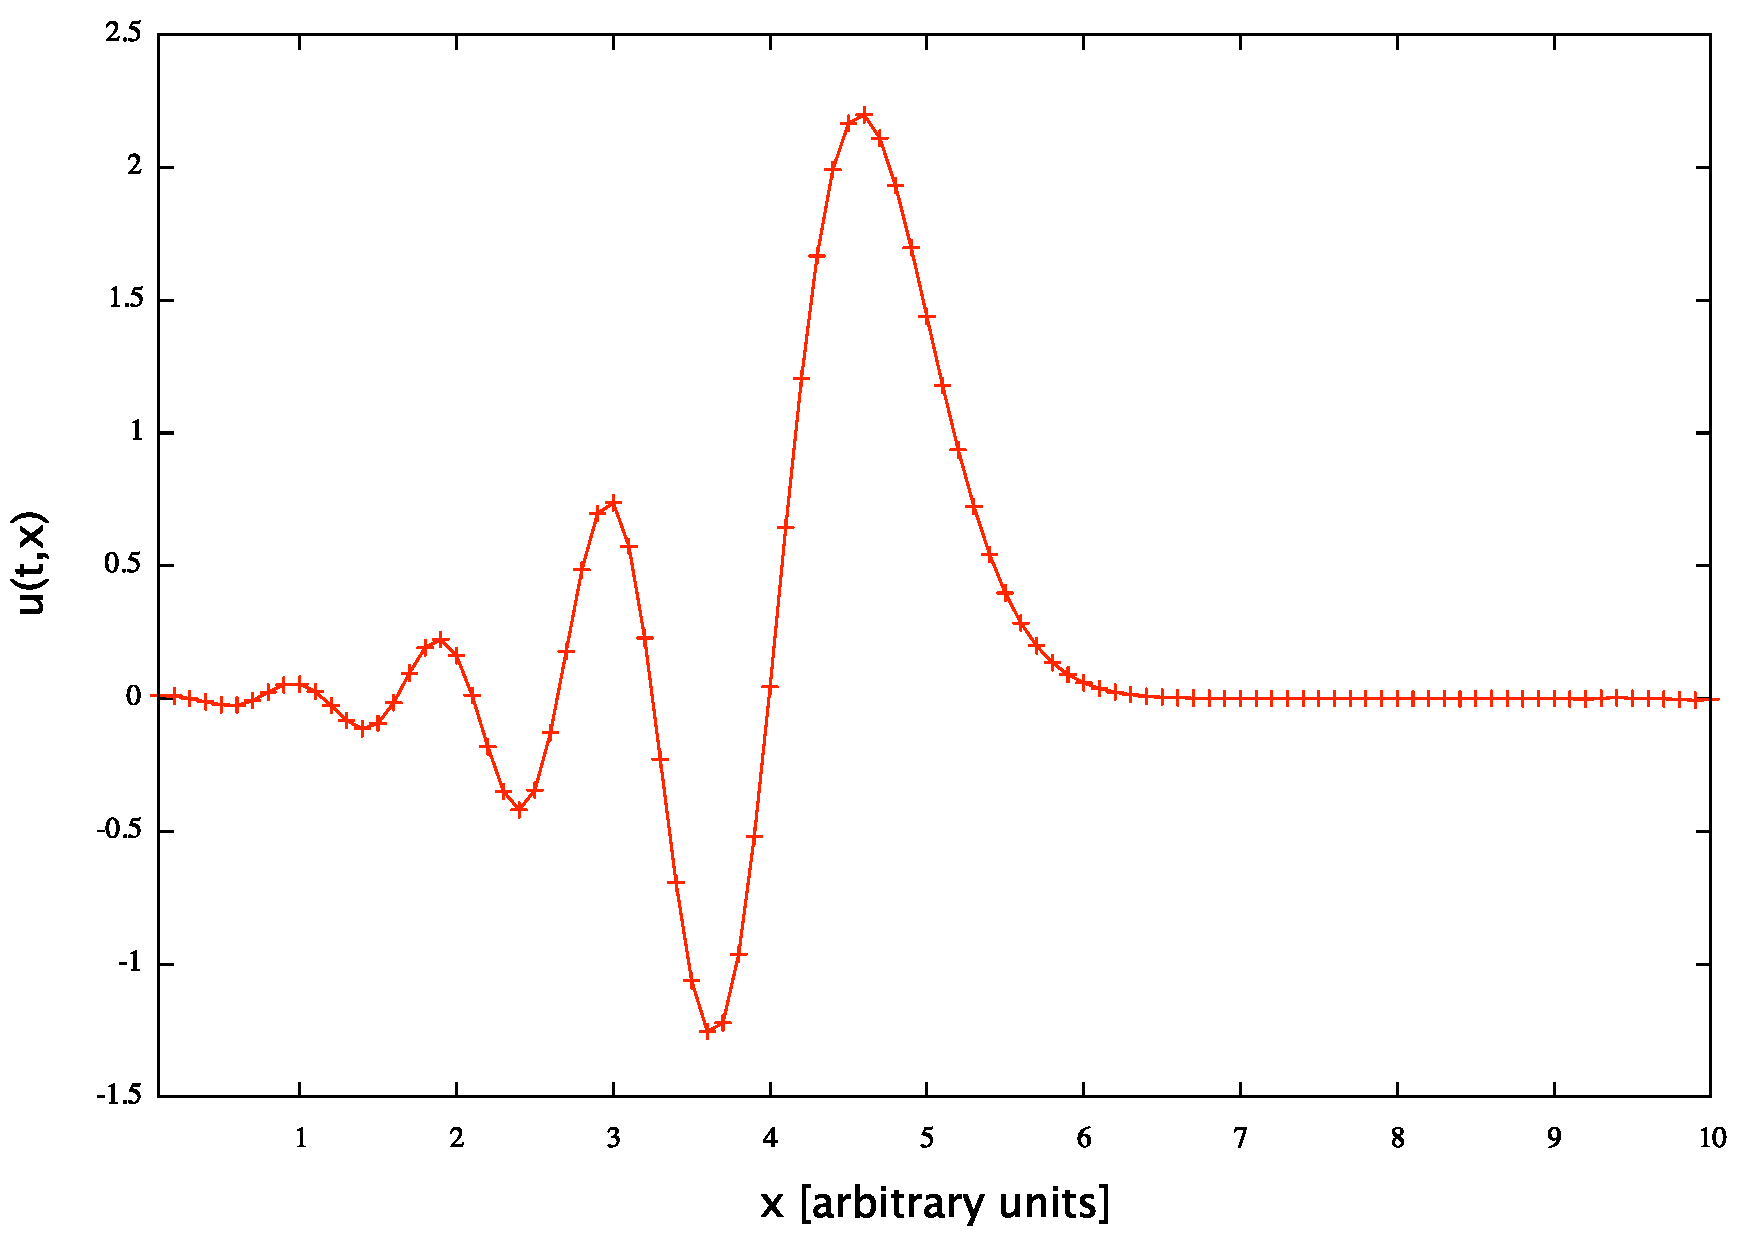
\includegraphics[scale=0.25]{ftcs_t10_cf05}}
\subfigure[$u(x,t=20)$ with $c_f=0.5$]
{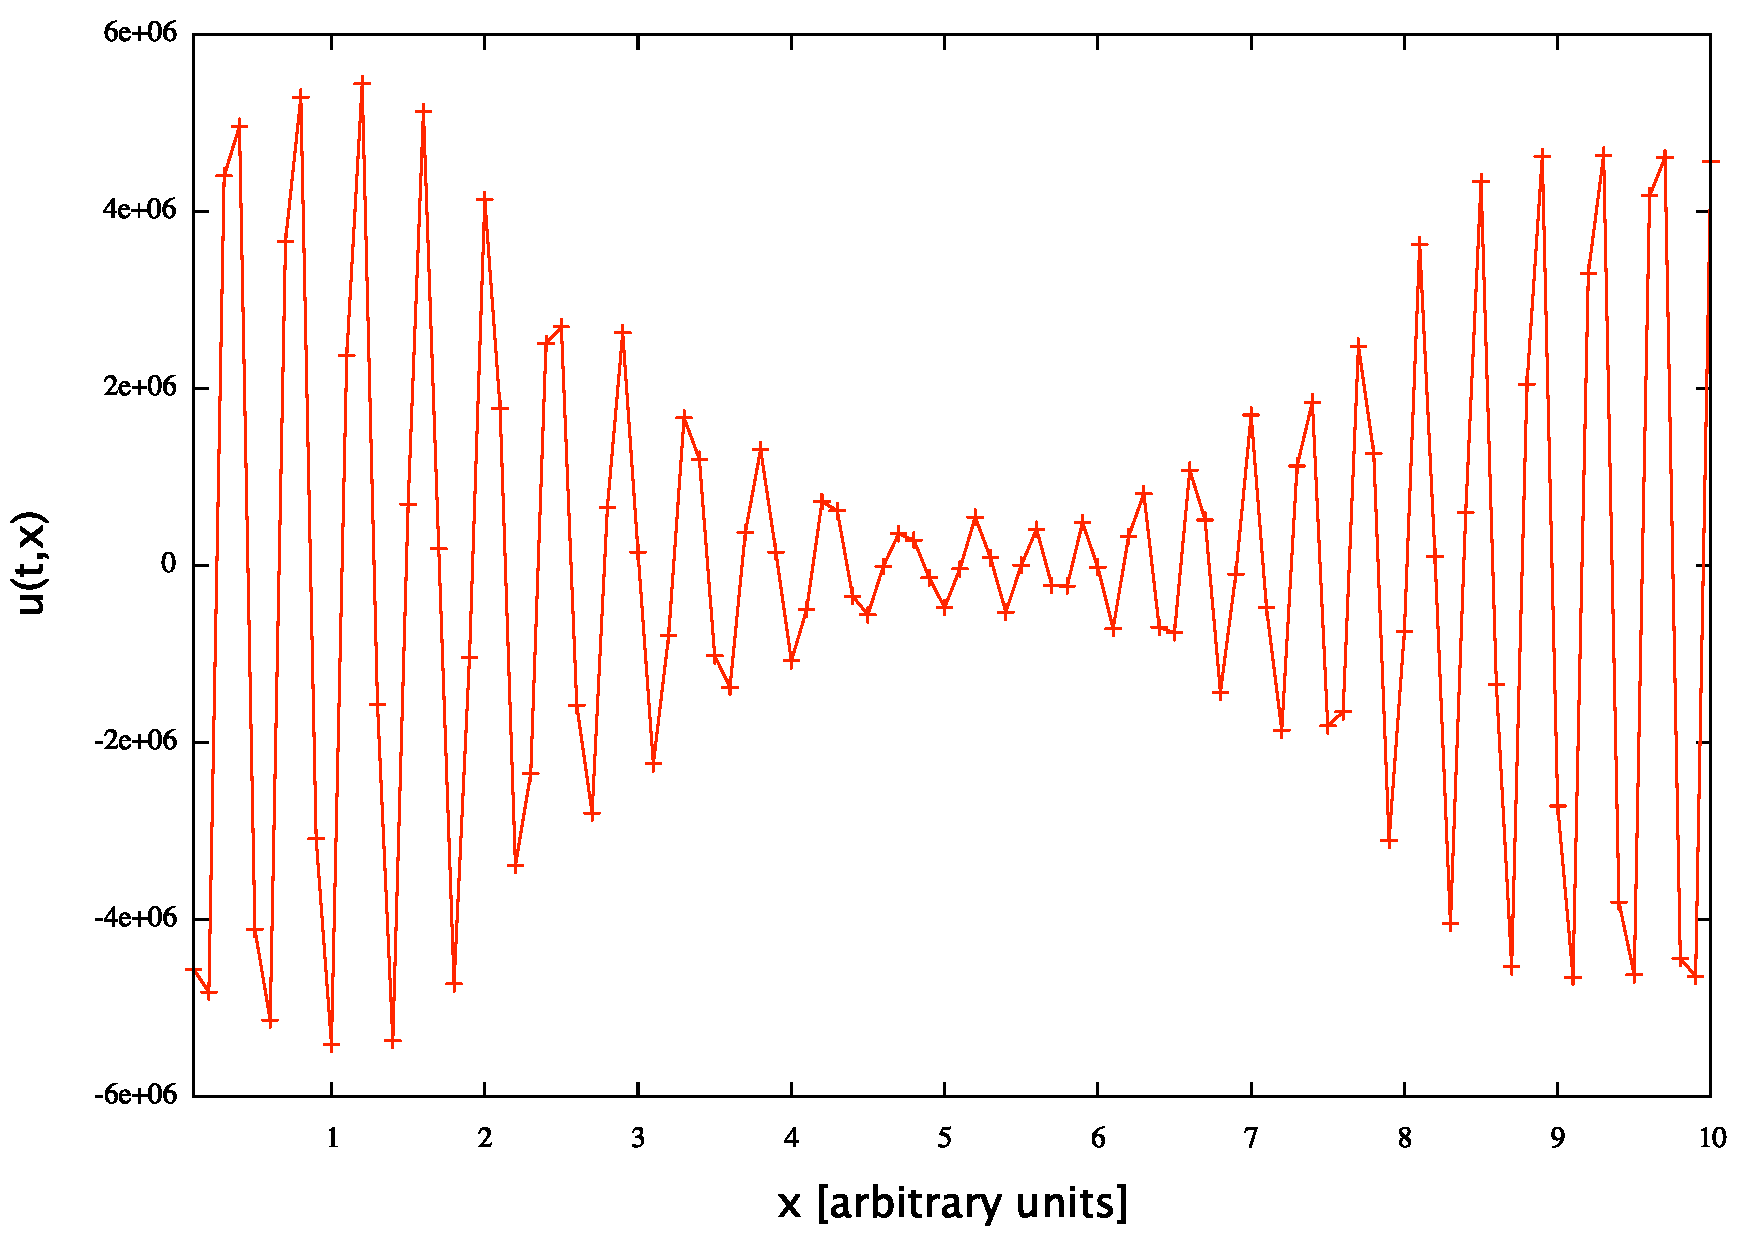
\includegraphics[scale=0.25]{ftcs_t20_cf05}}
%\caption{Results obtained with a gaussian wave with $J=101$ and $c_f=0.5$ using FTCS}
\end{figure} \ \\
In the case of $J=101$ points in the grid and $c_f=1$, instead, the following results are obtained:
\begin{figure}[!h]
\centering
\subfigure[$u(x,t=10)$ with $c_f=1$]
{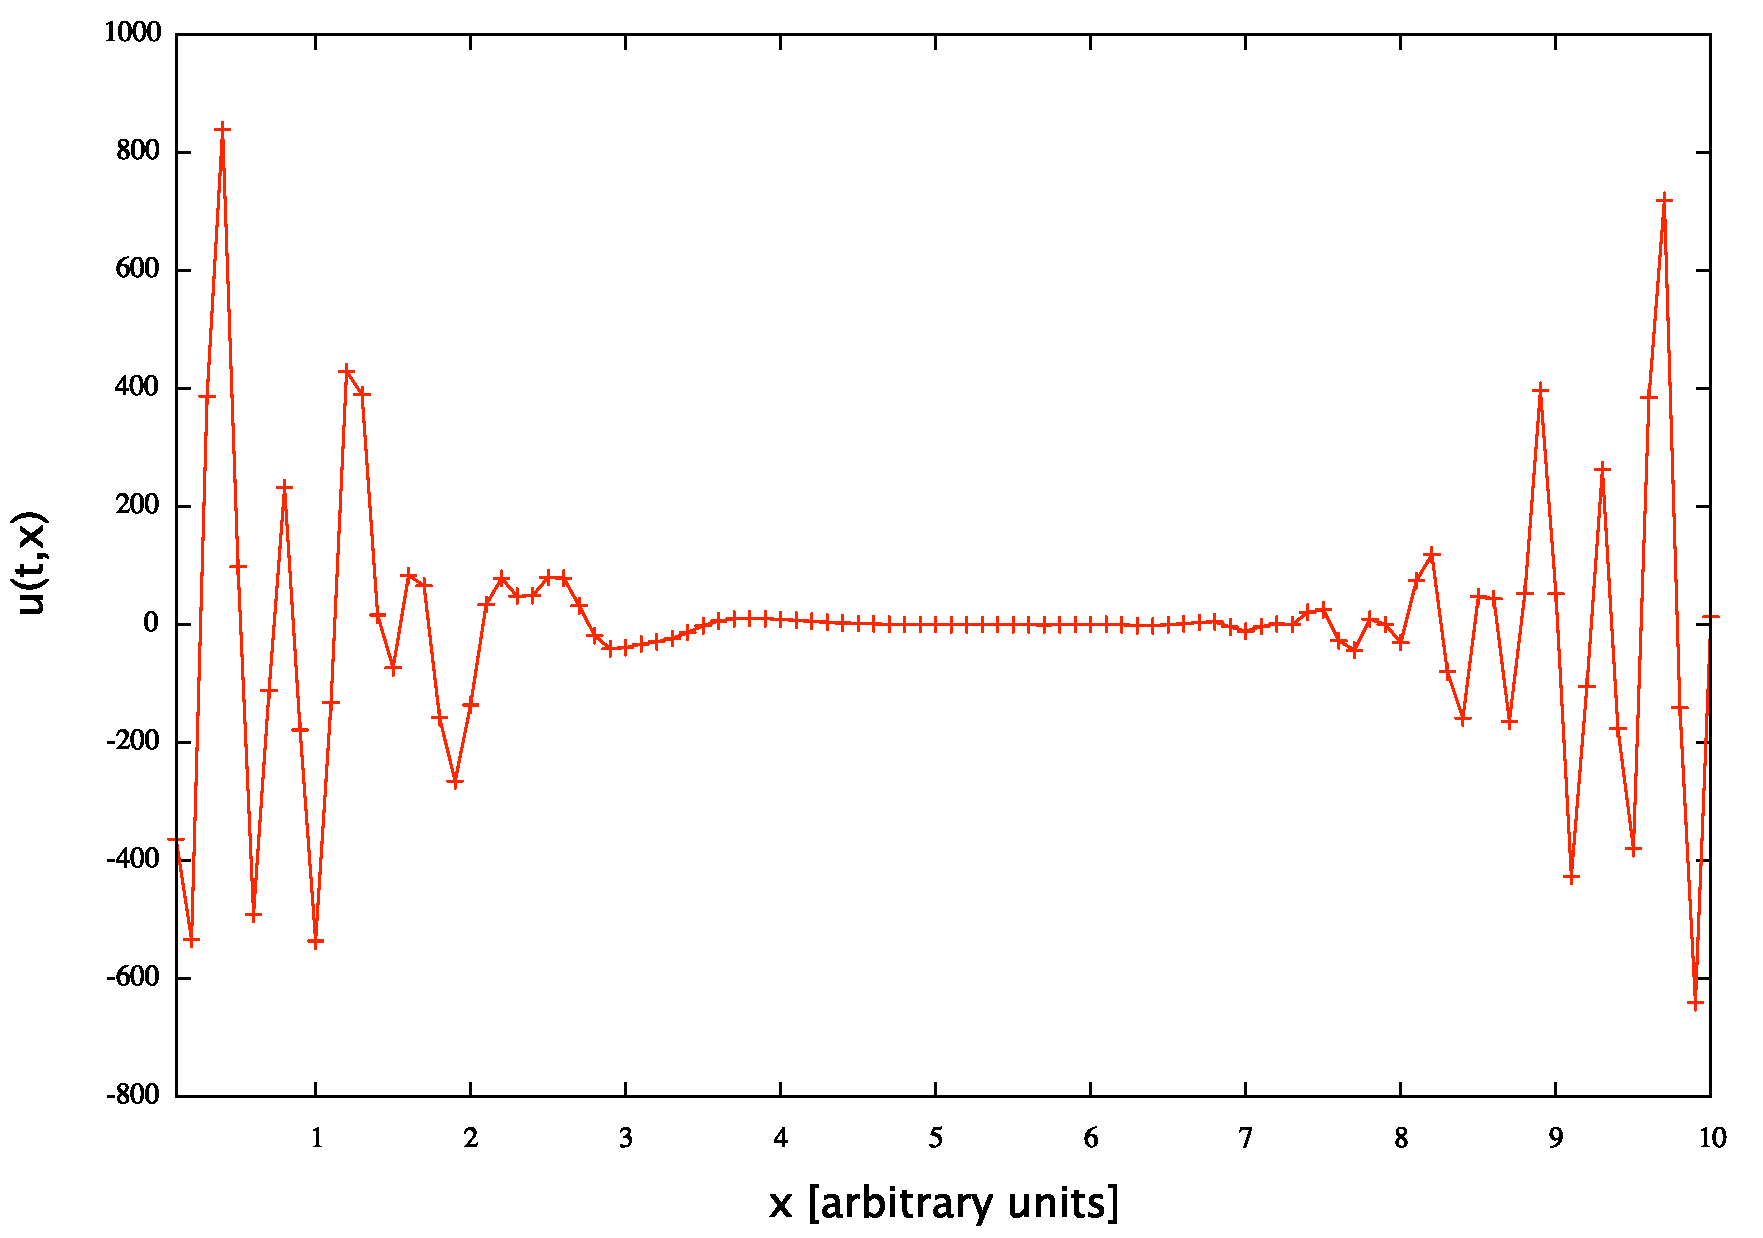
\includegraphics[scale=0.25]{ftcs_t10_cf1}}
\subfigure[$u(x,t=20)$ with $c_f=1$]
{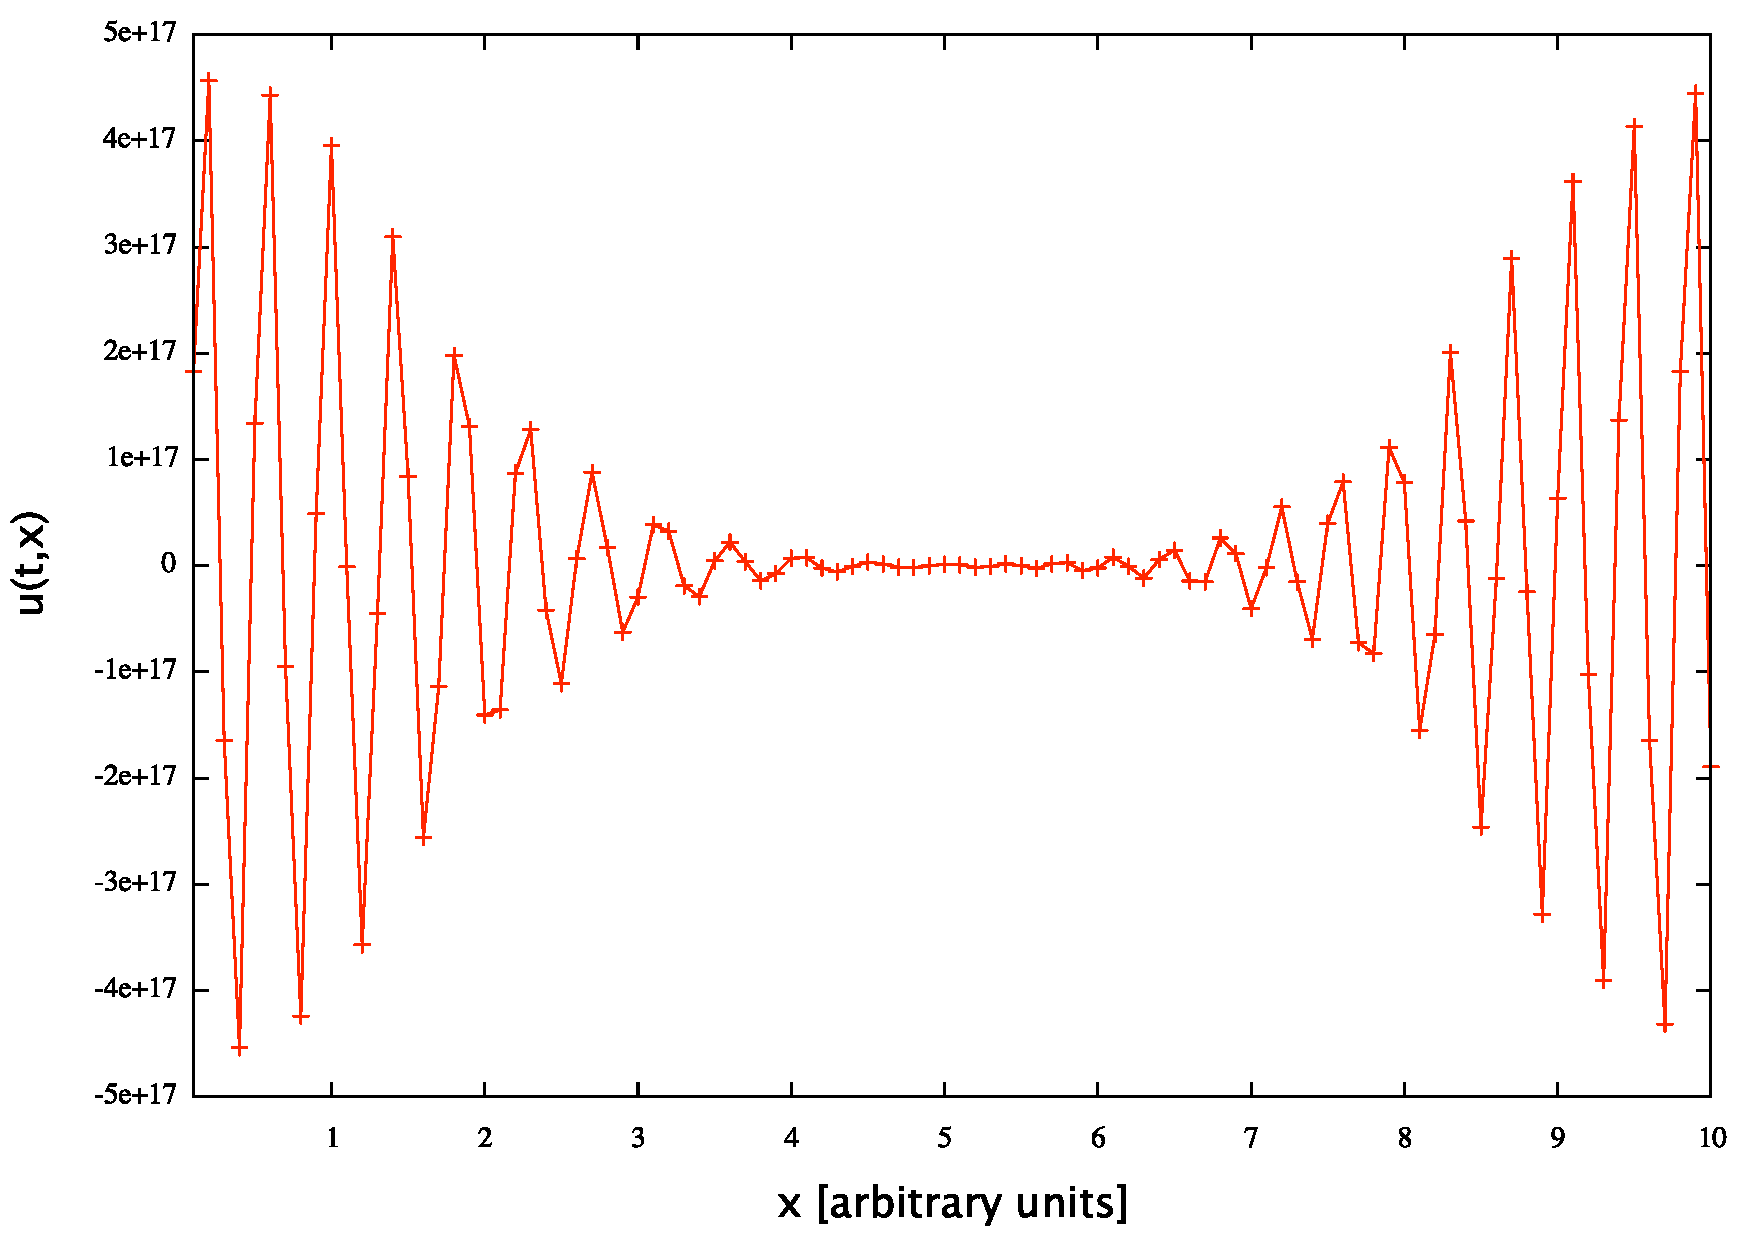
\includegraphics[scale=0.25]{ftcs_t20_cf1}}
%\caption{Results obtained with a gaussian wave with $J=101$ and $c_f=1$ using FTCS}
\end{figure}\ \\ \\
As one can easily figure out from the plots, the instability of the method completely destroys the solution even within $t=10$, that means that the method is quite useless for long lasting time evolutions, as initially stated. Another confirmation of this fact comes from the behaviour of the L2-norm in terms of time.
\begin{figure}[!h]
\centering
{\includegraphics[scale=0.4]{L2norm_ftcs}}
%\caption{Plot of the L2-norm (in logscale) with $J=101$ and $c_f=0.5,1$ using FTCS}
\end{figure}
It can clearly be observed that the norm is monotonously increasing and that it blows-up for for big $t$'s (with both $c_f=0.5$ and $c_f=1$), that is the error on the solution becomes infinite within a finite time. 
\\ \ \\
Different solutions of the avvection equation can be obtained using as starting function \eqref{1.2}. The computed results are shown in the following pictures. As can be clearly seen from the preceeding plots, the solution is already destroyed within the very first seconds of the simulation. 
\begin{figure}[!h]
\centering
\subfigure[$u(x,t=0.05)$ with $c_f=0.5,1$]
{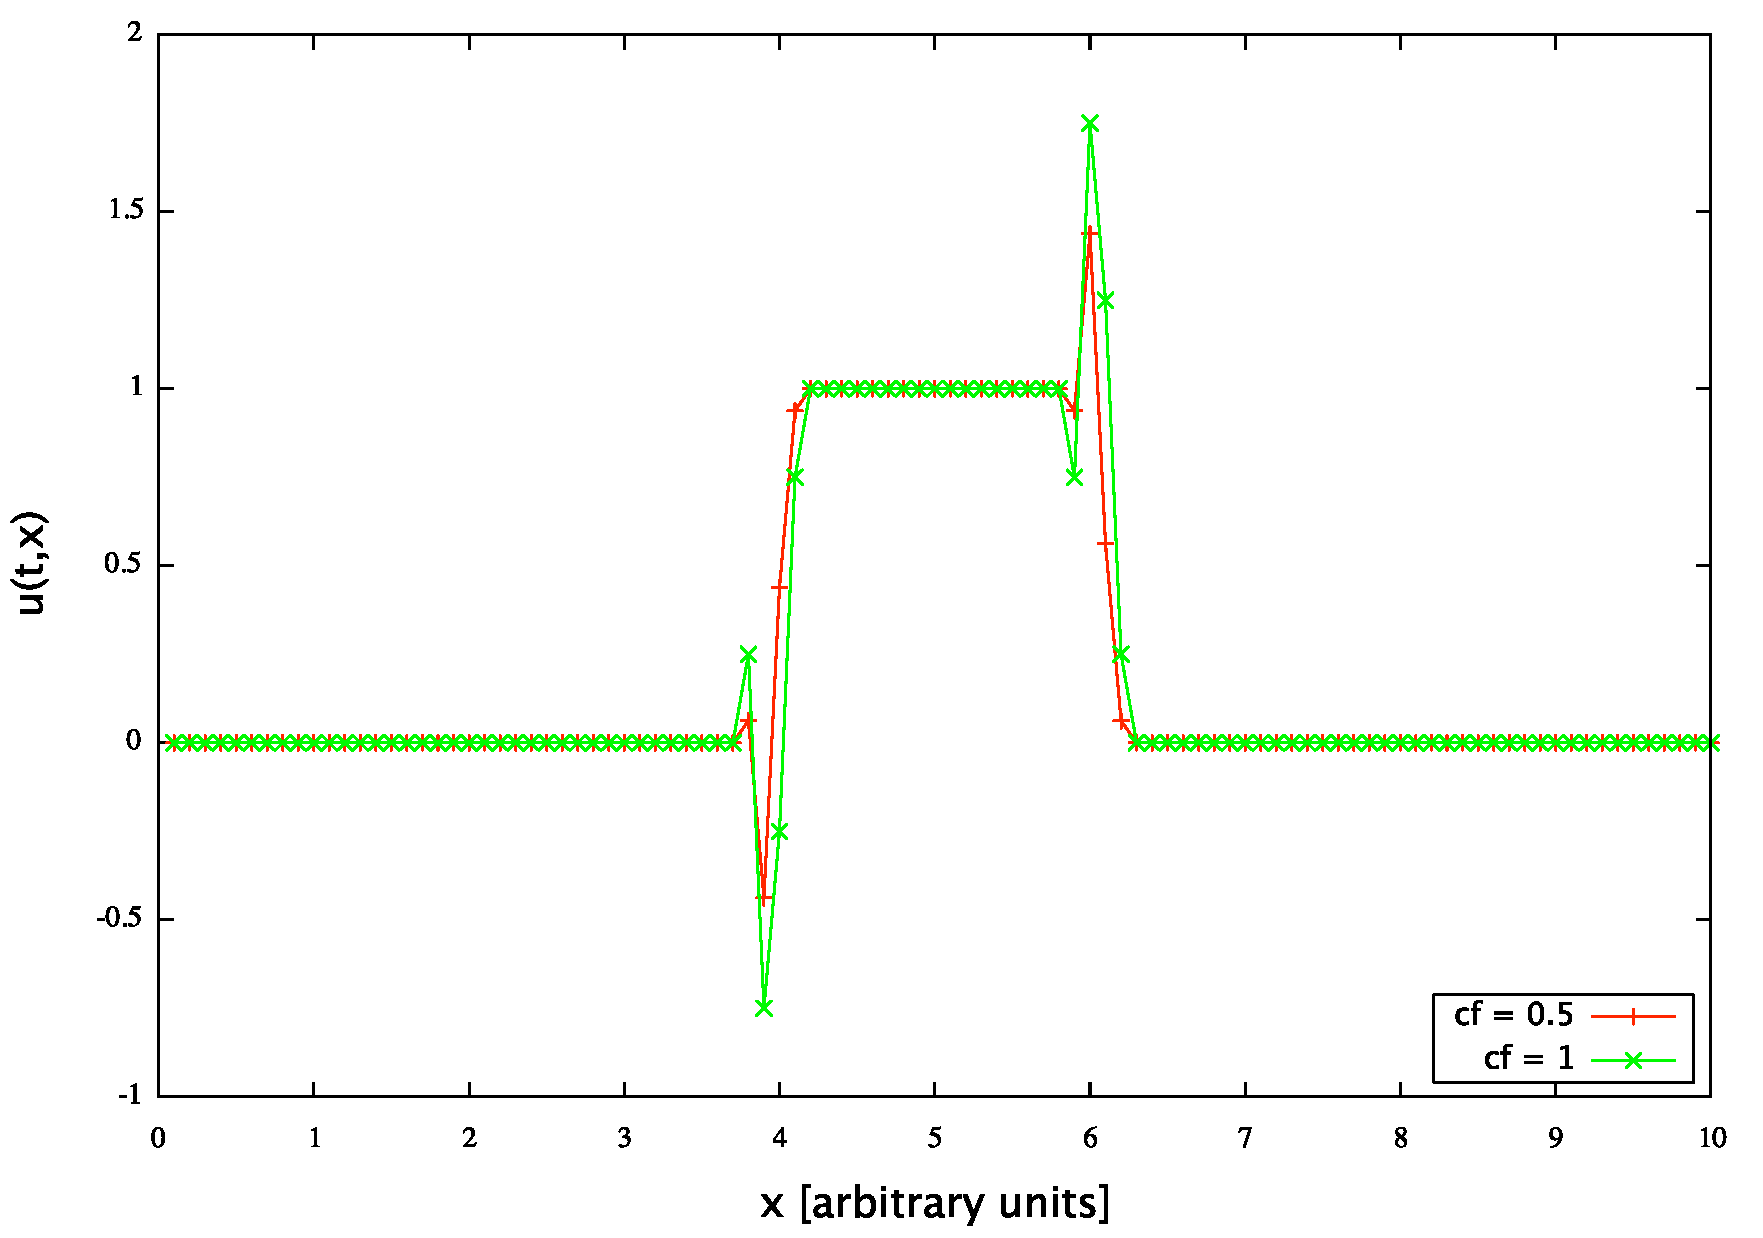
\includegraphics[scale=0.25]{ftcs_sw_tTSTEP}}
\subfigure[$u(x,t=1)$ with $c_f=0.5,1$]
{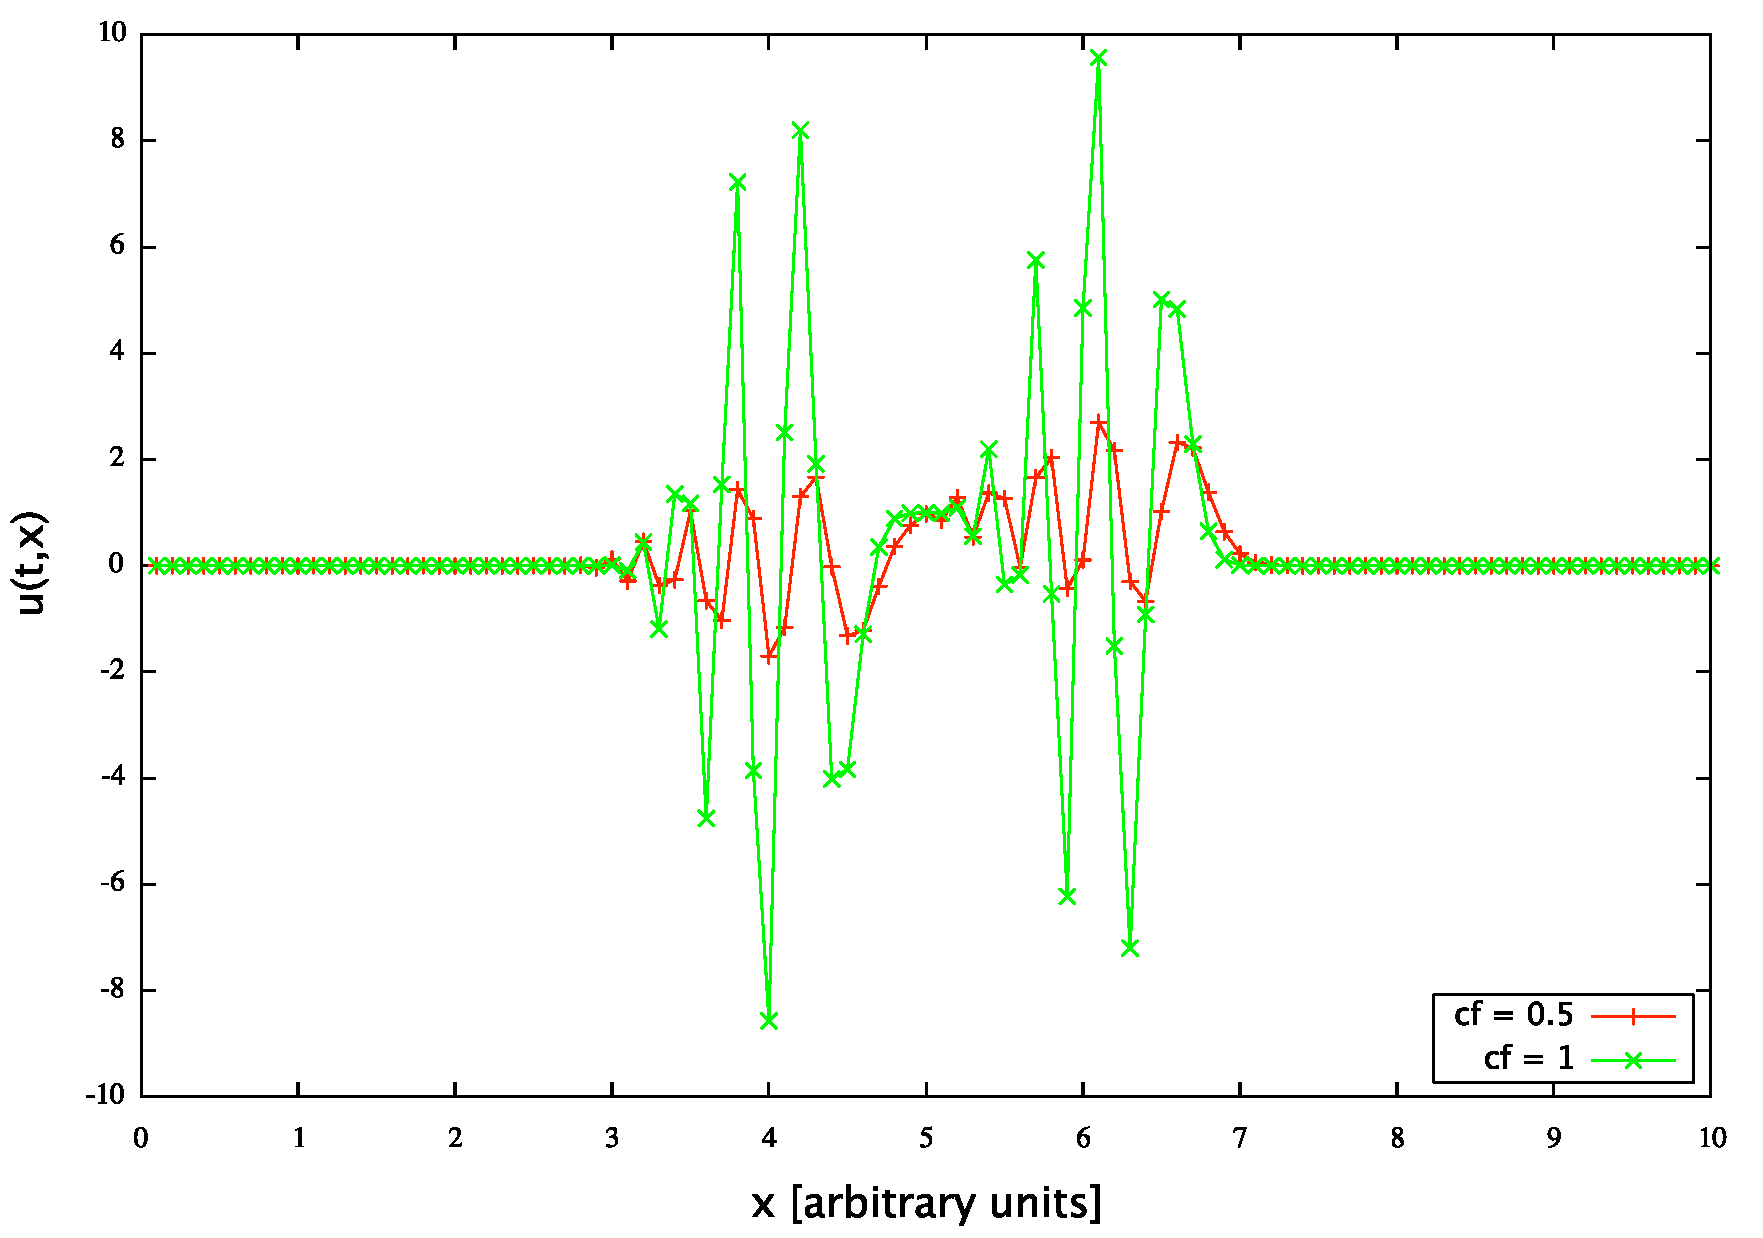
\includegraphics[scale=0.25]{ftcs_t1_sw}}
%\caption{Results obtained with a rectangular wave with $J=101$ and $c_f=0.5,1$ using FTCS}
\end{figure}
\ \\ \\
As a confirmation of this observation we can show the plot of the L2-norm in this case.
\begin{figure}[!h]
\centering
{\includegraphics[scale=0.4]{L2norm_ftcs_sw}}
%\caption{Plot of the L2-norm (in logscale) with $J=101$ and $c_f=0.5,1$ using FTCS}
\end{figure}
The value reached by the L2-norm at $t=20$ is even bigger then before, showing, definitively, that the FTCS is a non applicable method for the solution of the avvection equation. 

\section{The Leapfrog method}
The Leapfrog algorithm states that the solution for the avvection equation can be obtained as follows:
\begin{equation}
u_j^{n+1} = u_j^{n-1} - a\frac{\Delta t}{\Delta x} ( u_{j+1}^n - u_{j-1}^n)
\end{equation}
As can be easily seen, one of the fundamental differences between this and the former method lies in the fact that one need to double the storage space in order to compute the solution, because the $n+1$ step depends on the $n$ and the $n-1$ steps. Using the Von Neumann stability analysis one finds that leapfrog is a stable method as long as $|a|\frac{\Delta t}{\Delta x} = c_f < 1$. Therefore, let's look at the obtained solutions implementing the leapfrog algorithm in different conditions.
\begin{figure}[!h]
\centering
\subfigure[$u(x,t=10)$ with $c_f=0.5$]
{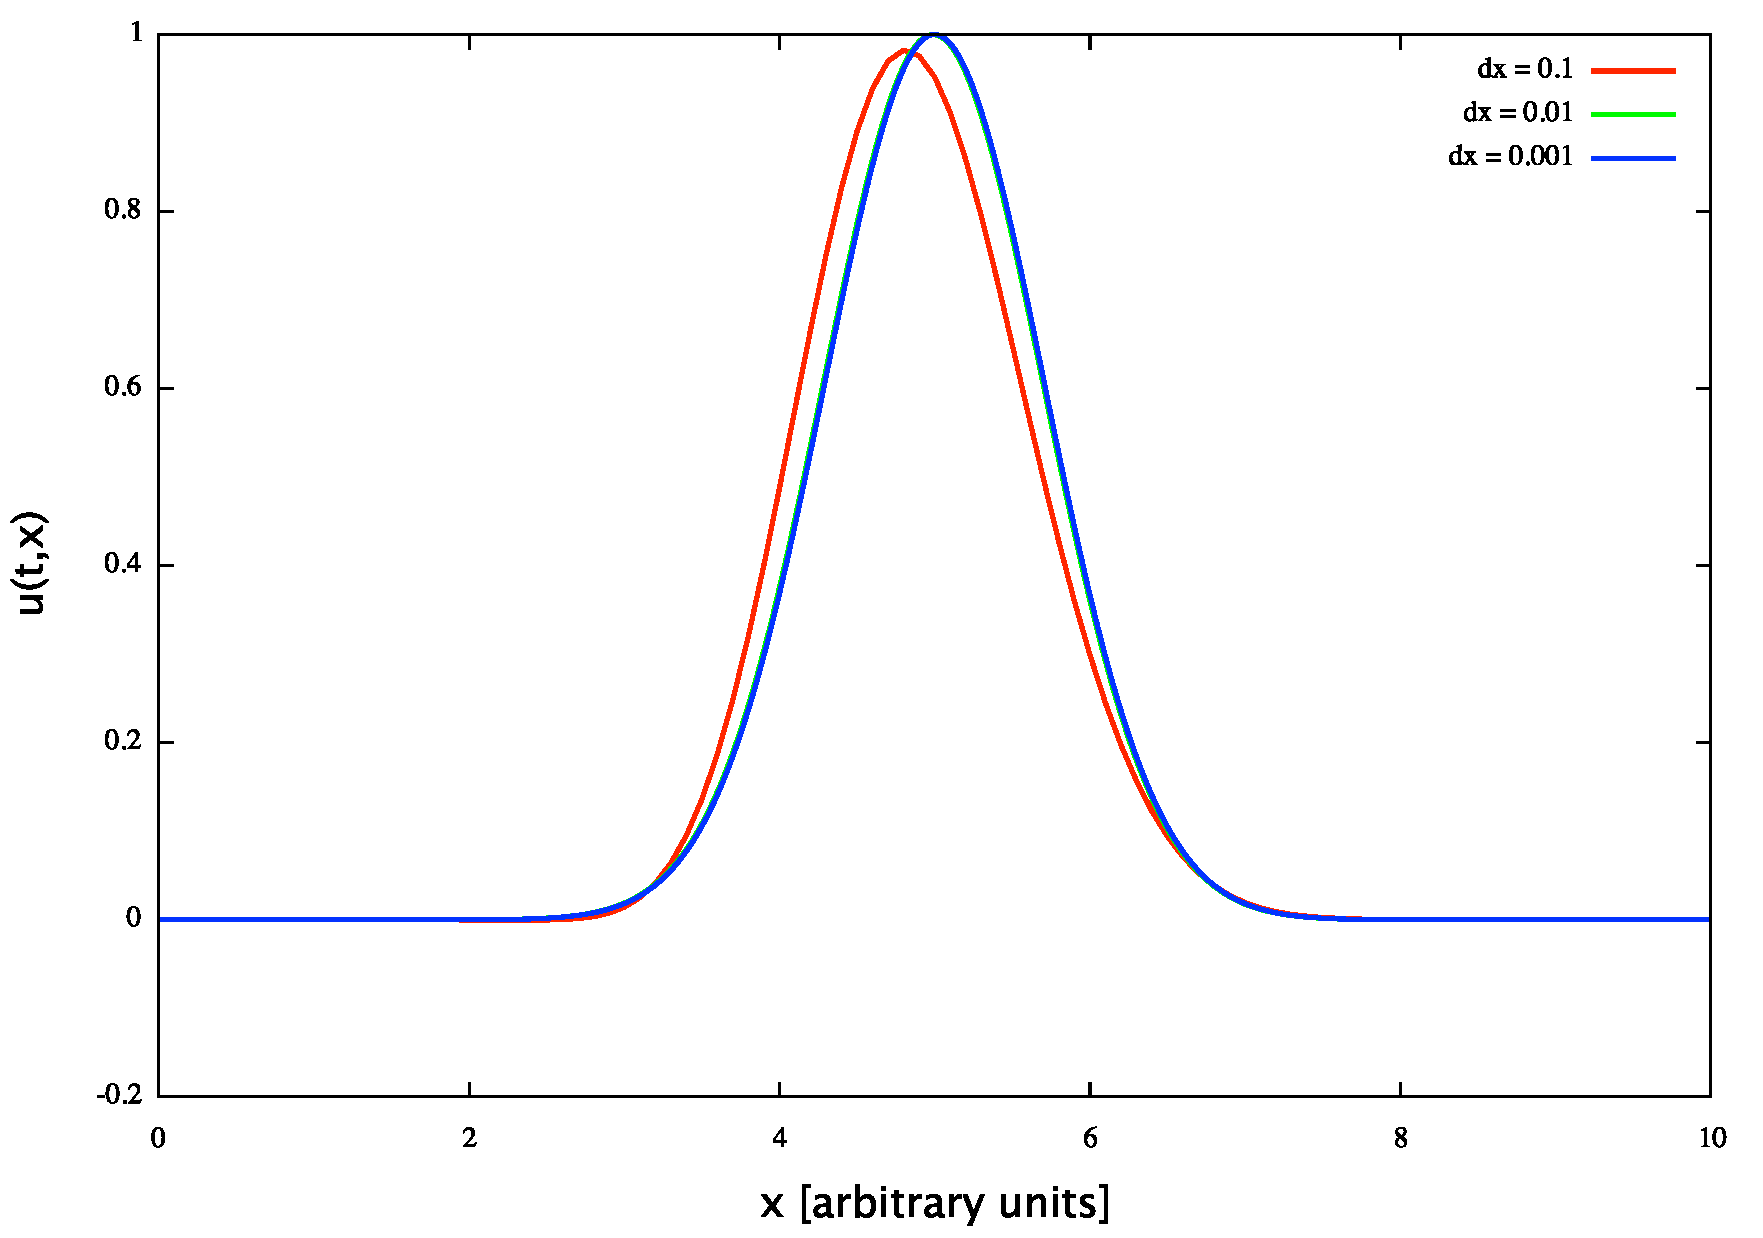
\includegraphics[scale=0.25]{good_img/lf_cf05_t10_g}}
\subfigure[$u(x,t=20)$ with $c_f=0.5$]
{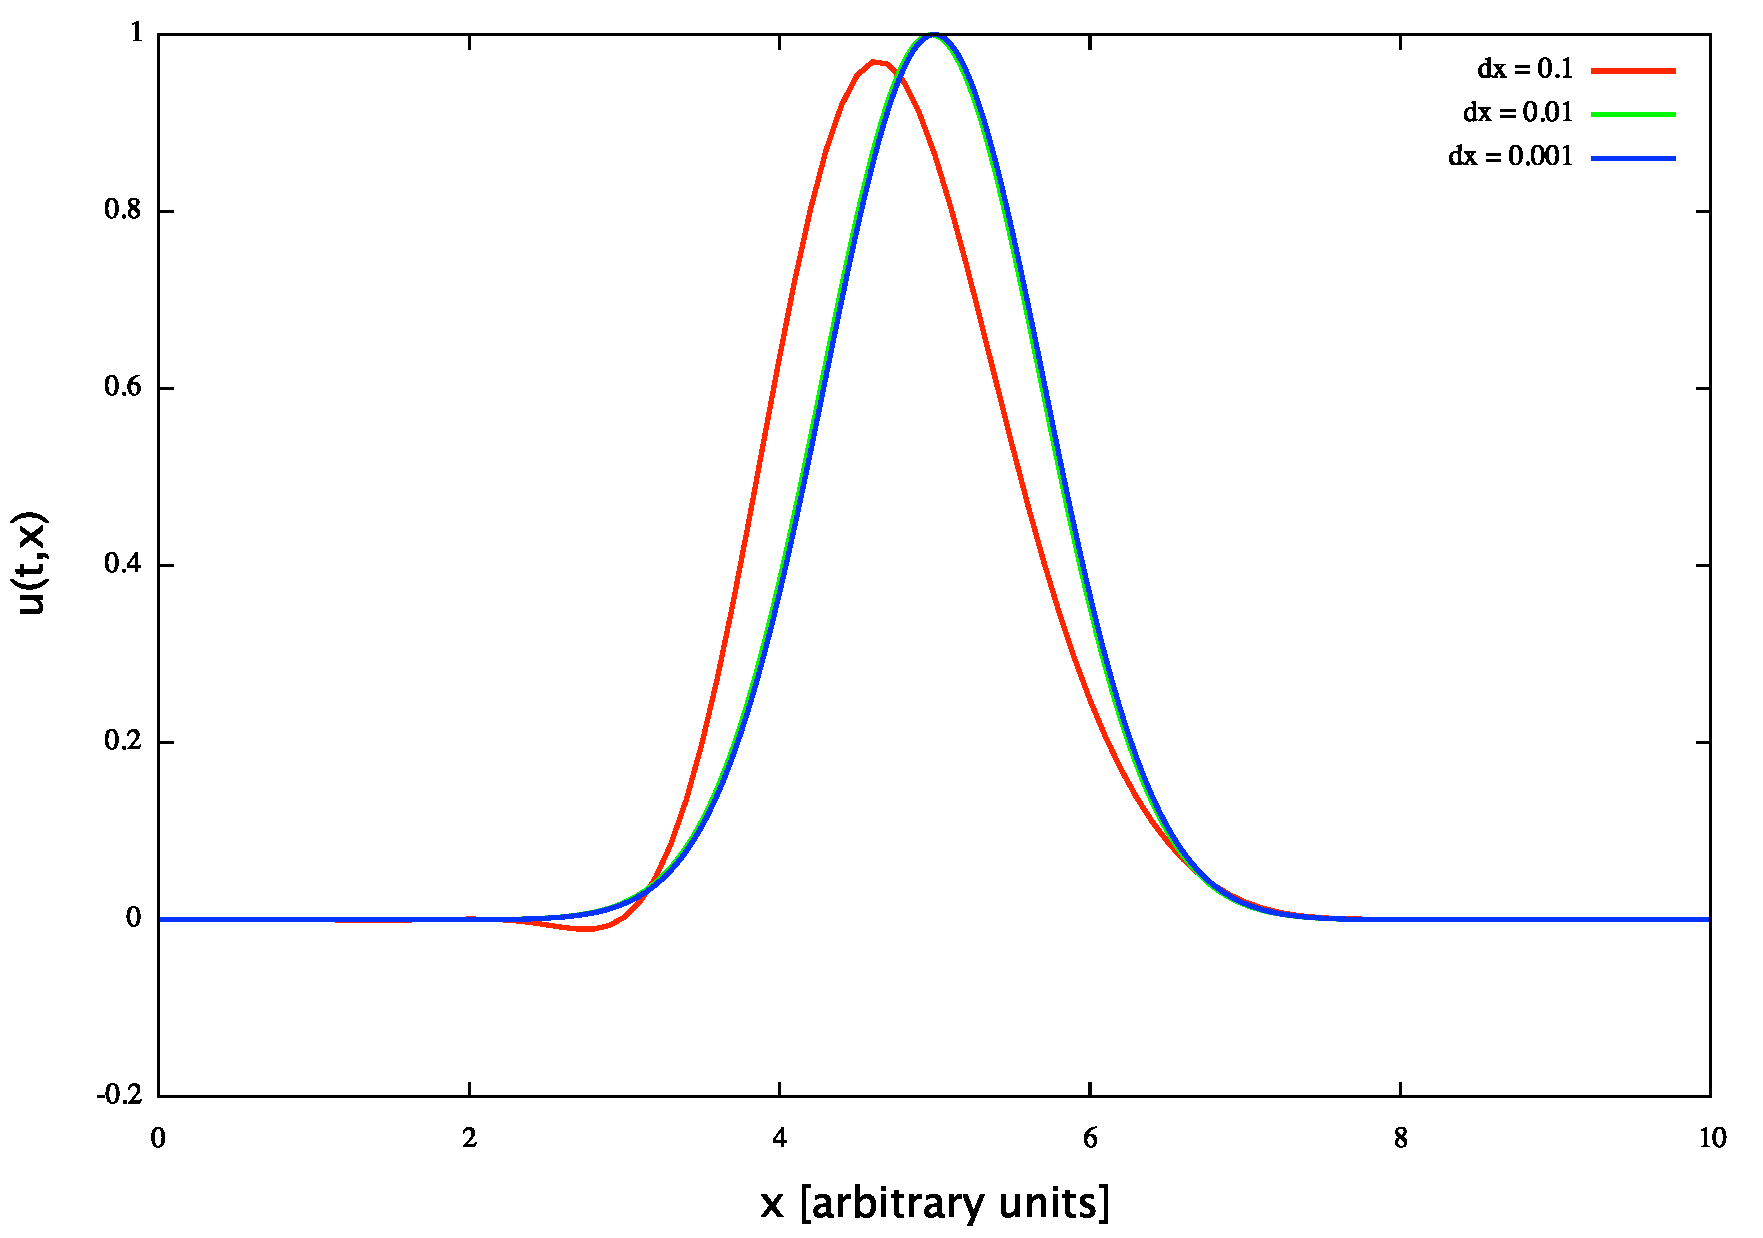
\includegraphics[scale=0.25]{good_img/lf_cf05_t20_g}}
\subfigure[$u(x,t=10)$ with $c_f=1$]
{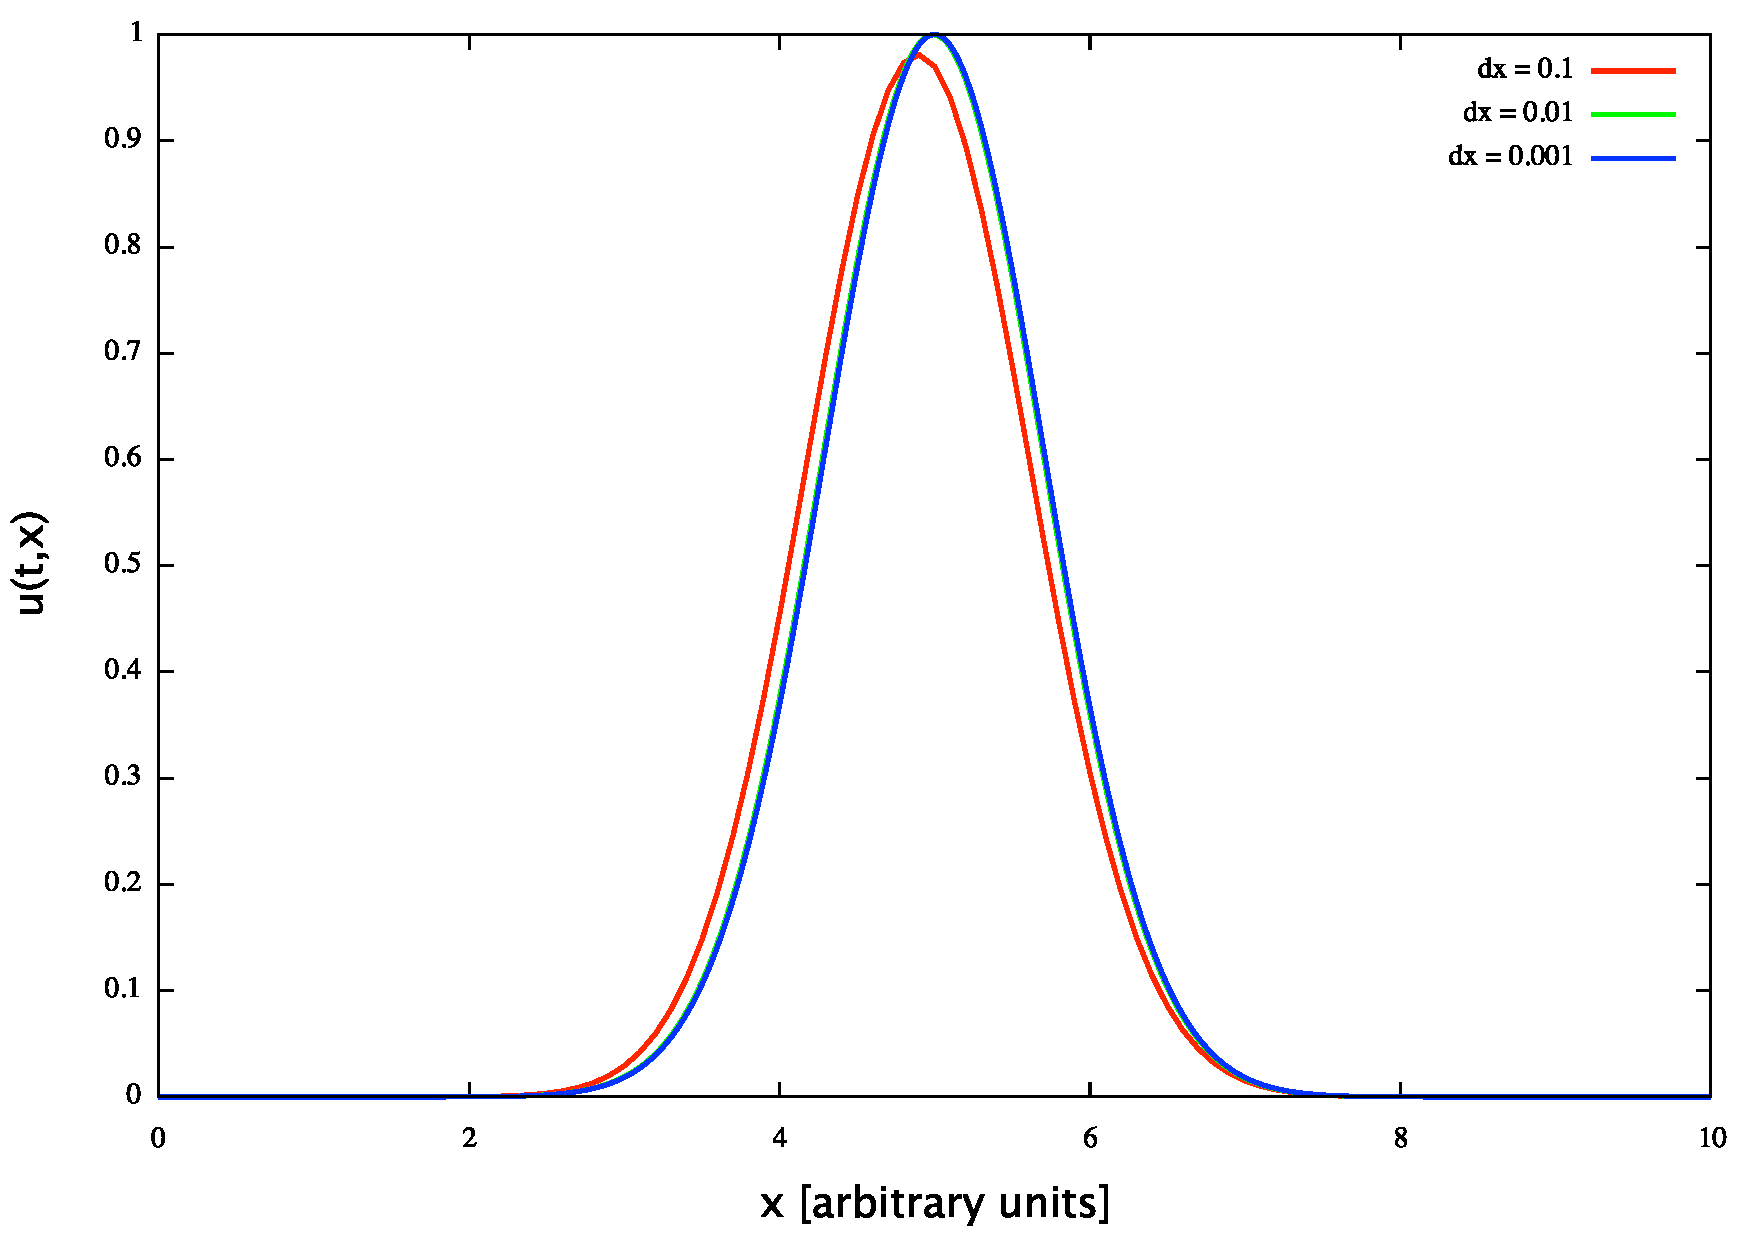
\includegraphics[scale=0.25]{good_img/lf_cf1_t10_g}}
\subfigure[$u(x,t=20)$ with $c_f=1$]
{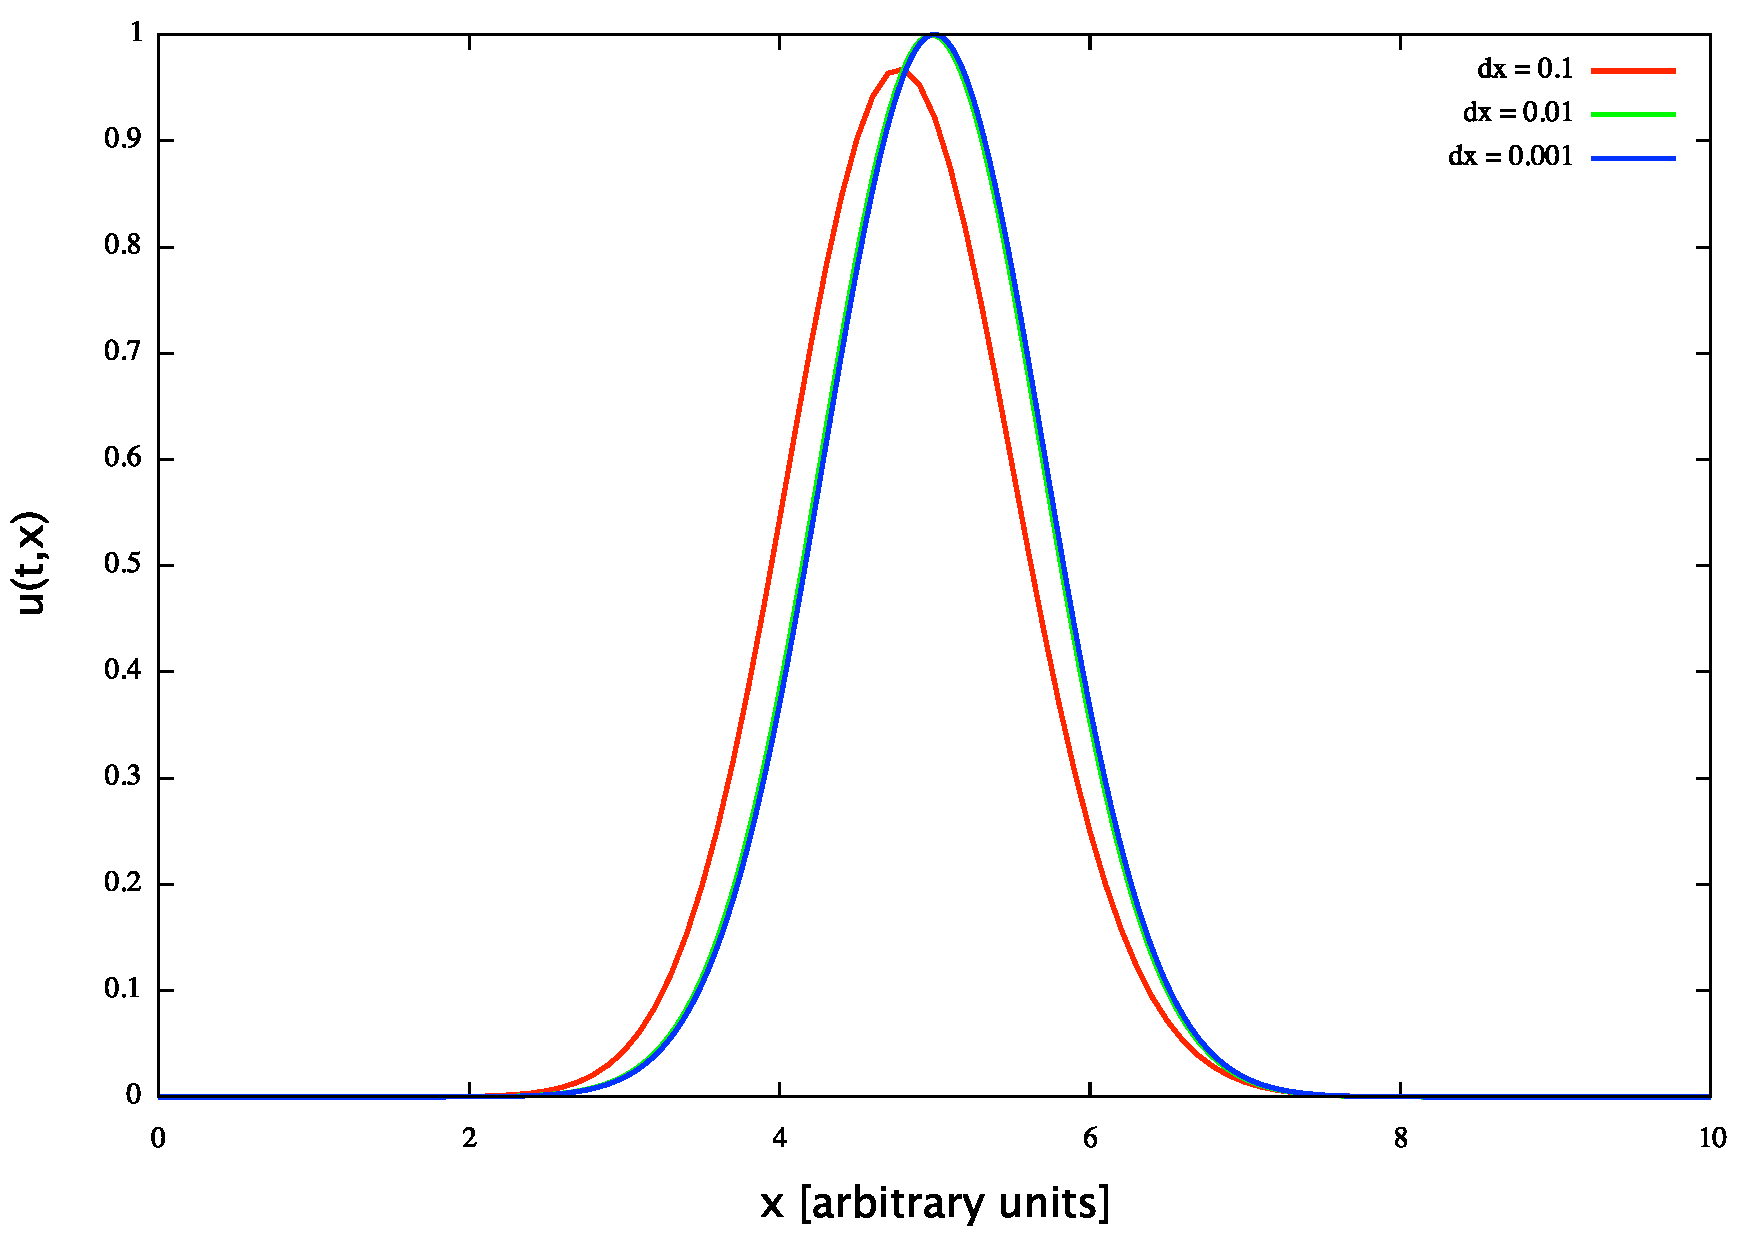
\includegraphics[scale=0.25]{good_img/lf_cf1_t20_g}}
%\caption{Results obtained with a gaussian wave with $J=101,1001,10001$, $c_f=0.5,1$ and $T = 10,20$ using leapfrog method}
\end{figure}
One sees that the method is indeed stable, and the errors for $J=101$ are due only to the fact that the spacing of the mesh is too big. %Therefore, the Leapfrog algorithm with $\Delta x \leq 0.01$ and gaussian initial condition is a reliable method to solve the avvection equation. 
About the square wave initial condition the following results have been obtained. 
\begin{figure}[!h]
\centering
\subfigure[$u(x,t)$ with $c_f=0.5$ and $\Delta x = 0.1$]
{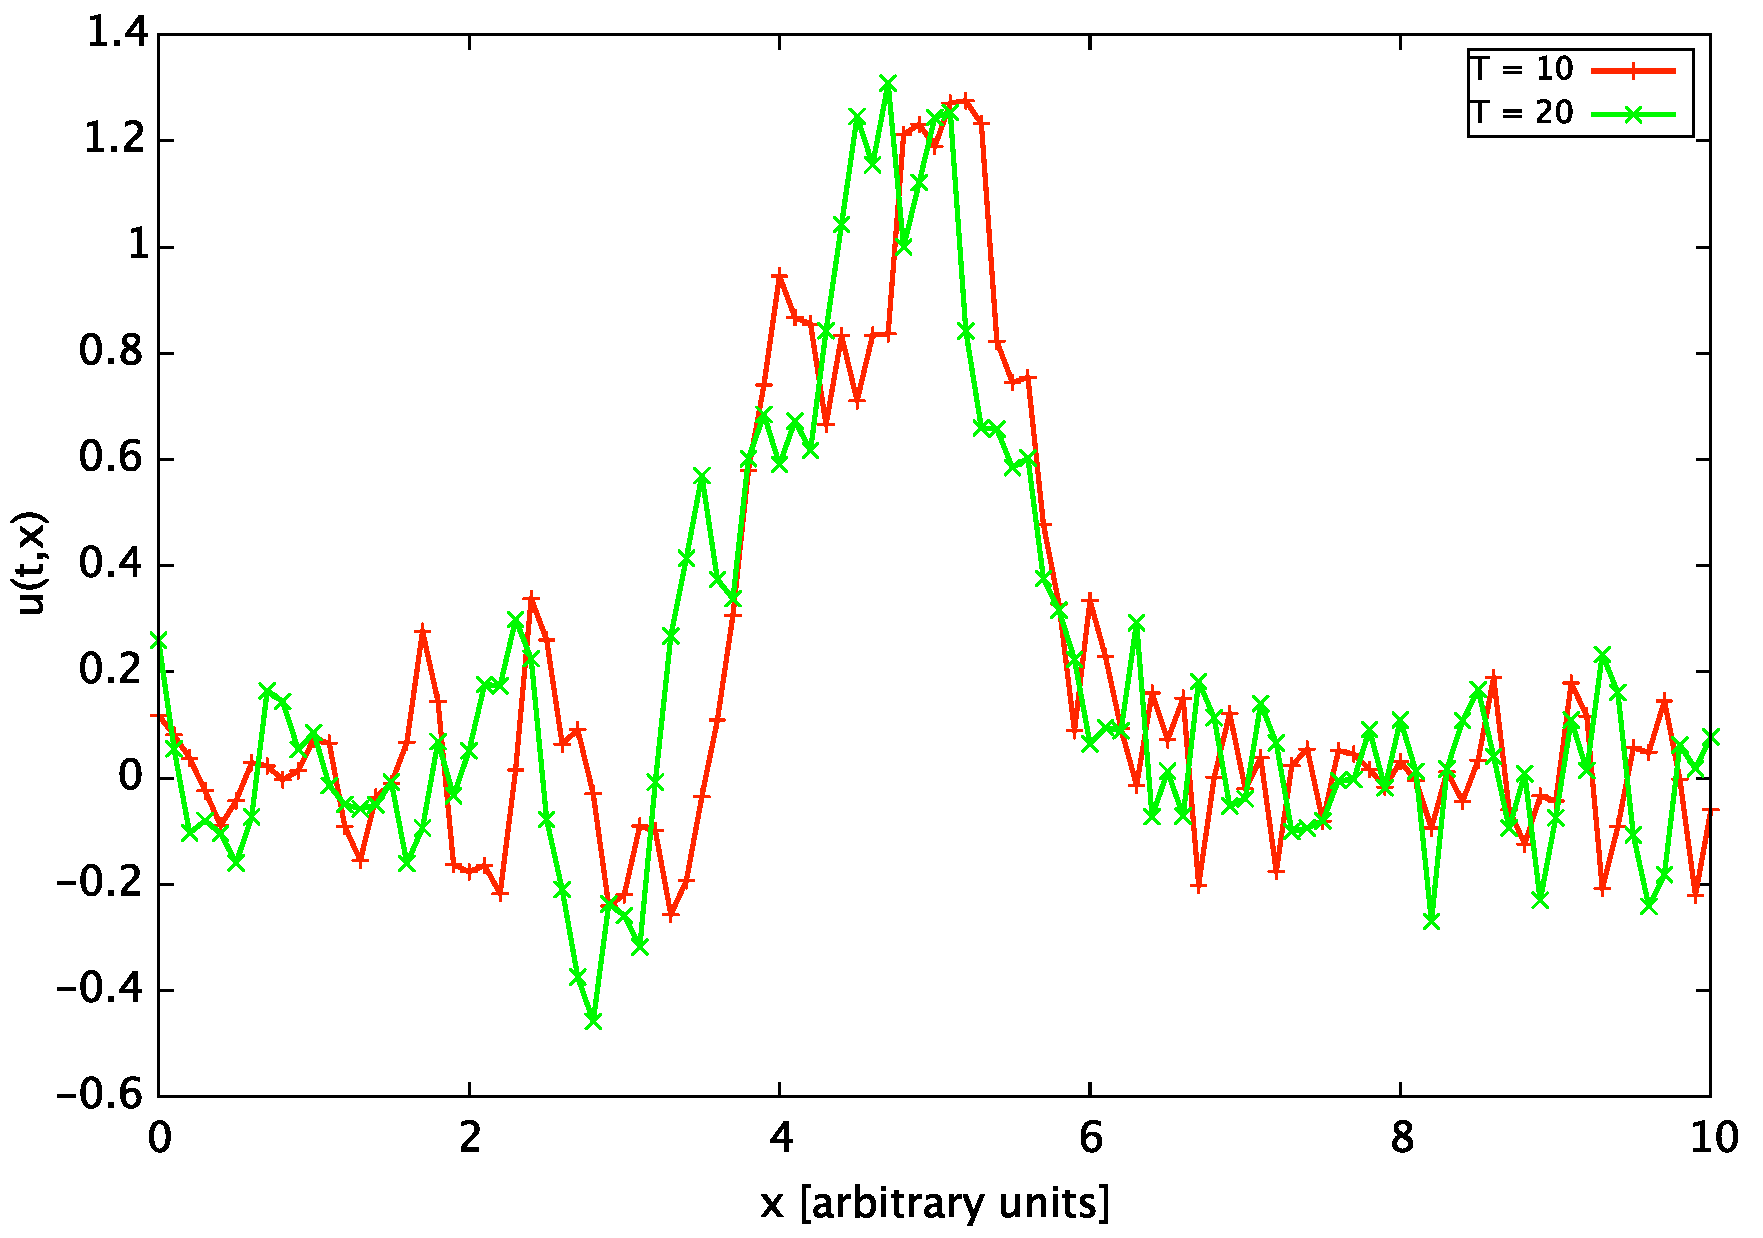
\includegraphics[scale=0.25]{good_img/lf_cf05_dx01_s}}
\subfigure[$u(x,t=10)$ with $c_f=0.5$ and $\Delta x = 0.01$]
{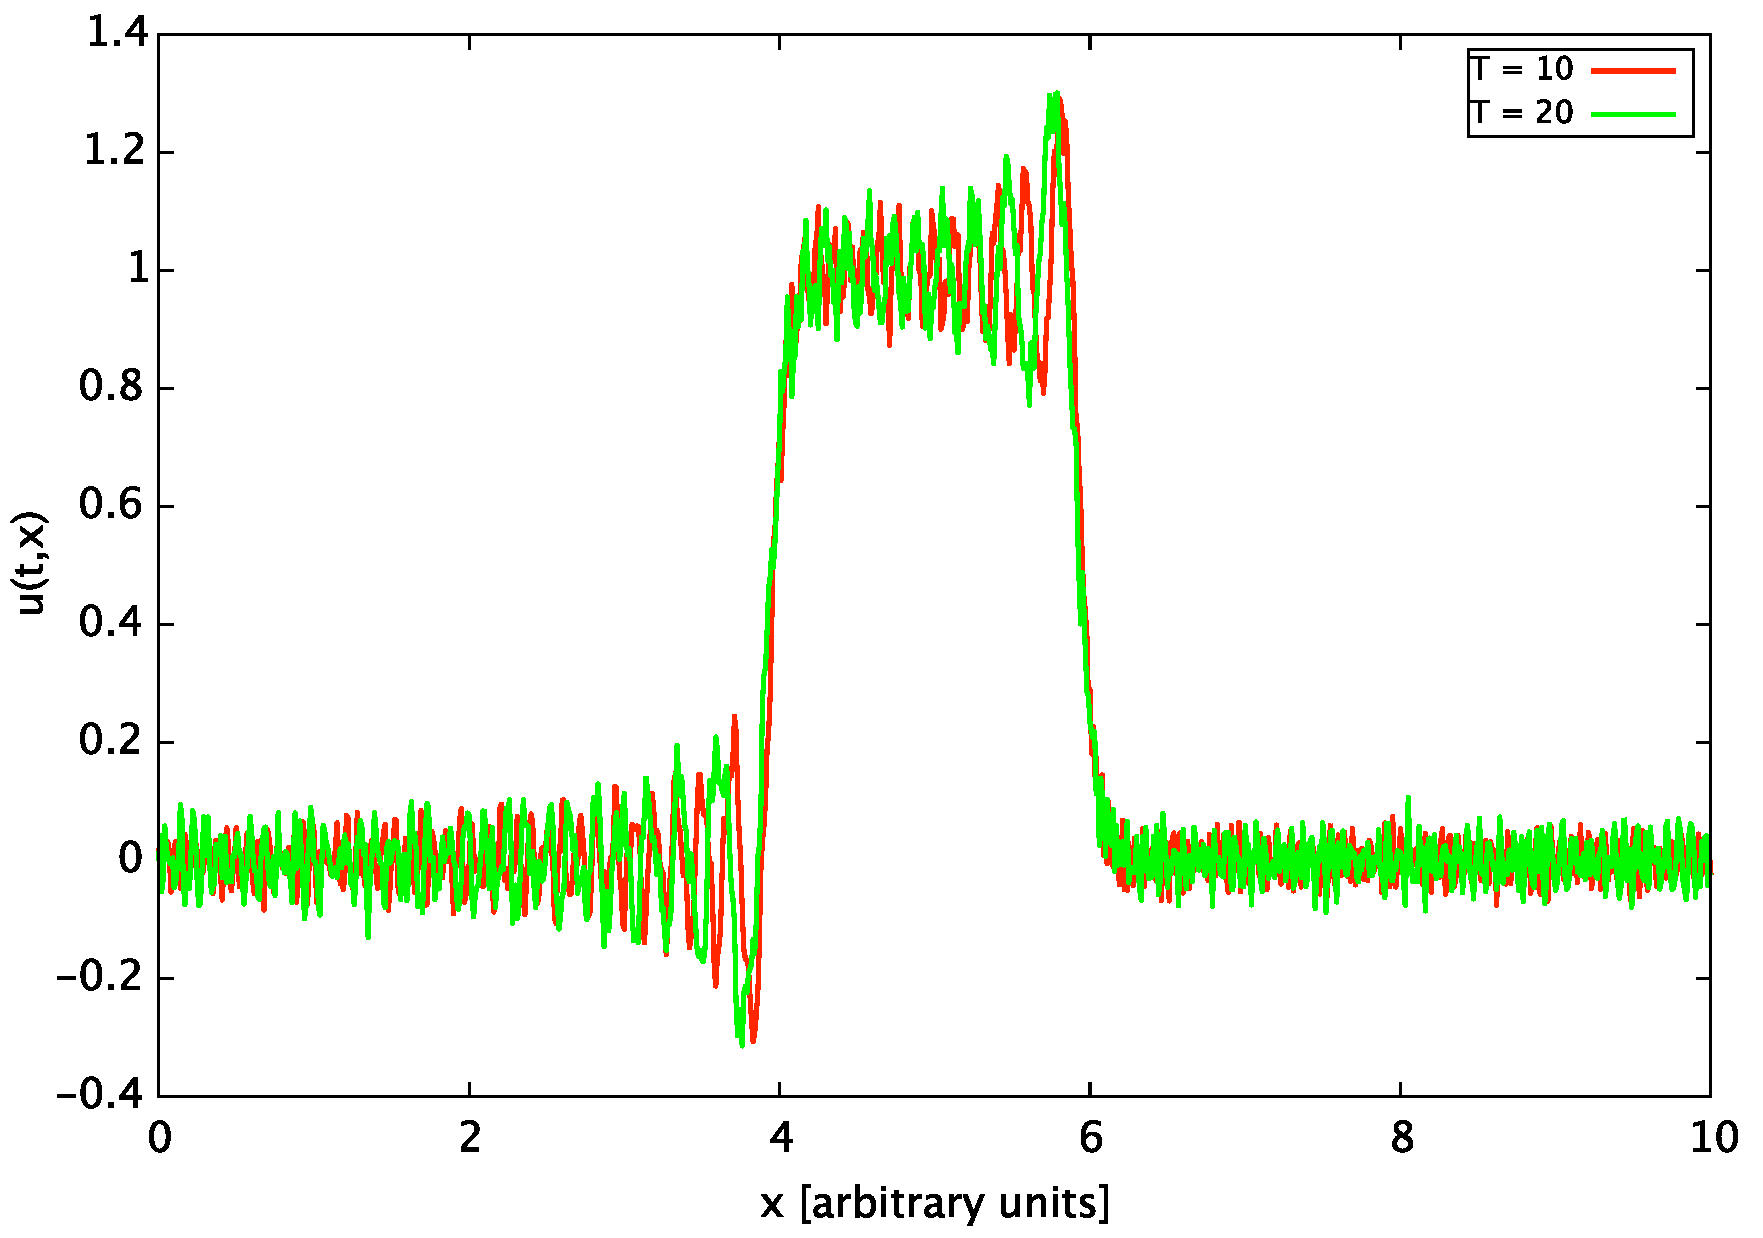
\includegraphics[scale=0.25]{good_img/lf_cf05_dx001_s}}
\end{figure}
It is clear that leapfrog is not a good method to integrate advection equation in case of square wave initial condition. The problem lies in the fact that the algorithm does not take care of the discontinuity in the derivative of the initial condition, therefore propagating the wave wrongly. Even with a different Courant factor the problem is not solved.
\begin{figure}[!h]
\centering
\subfigure[$u(x,t=10)$ with $c_f=1$ and $\Delta x = 0.1$]
{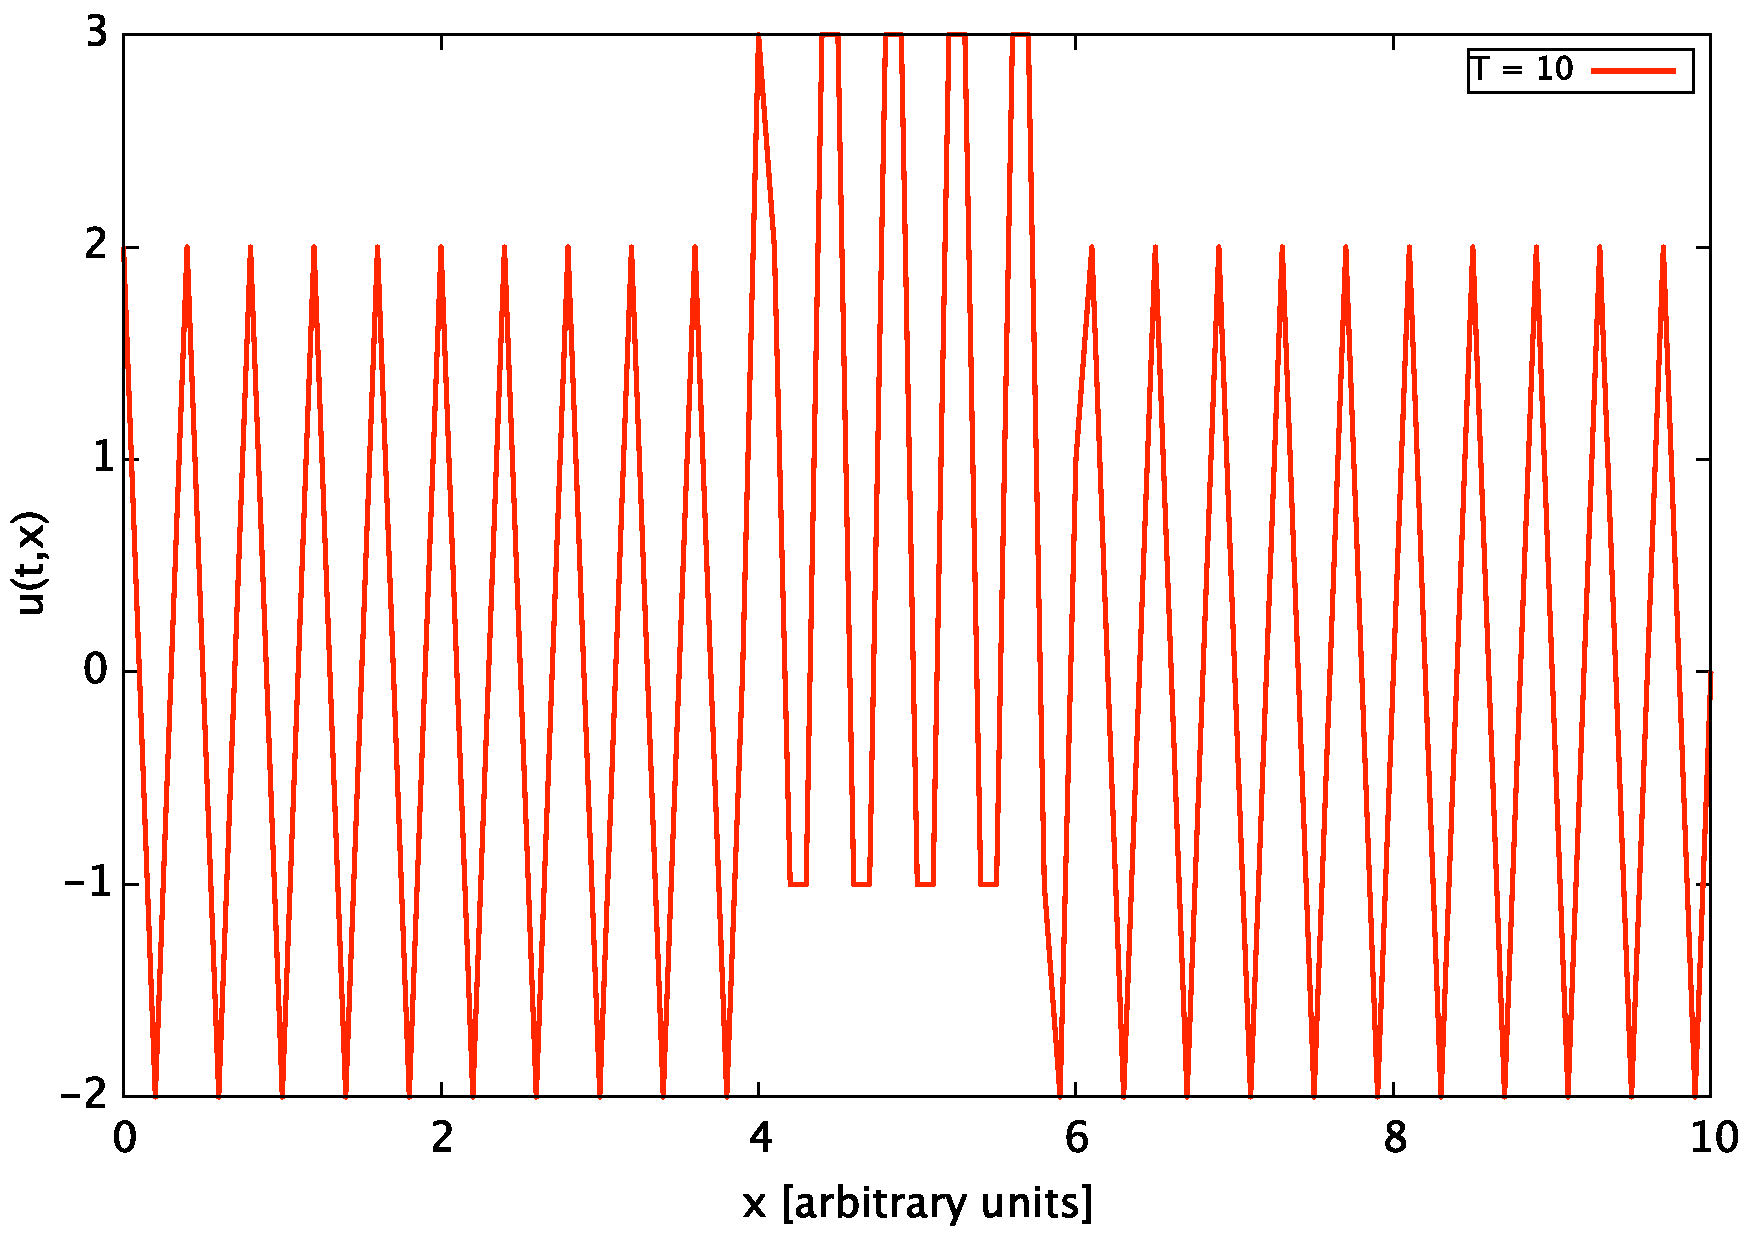
\includegraphics[scale=0.25]{good_img/lf_cf1_t10_dx01_s}}
\subfigure[$u(x,t=20)$ with $c_f=1$]
{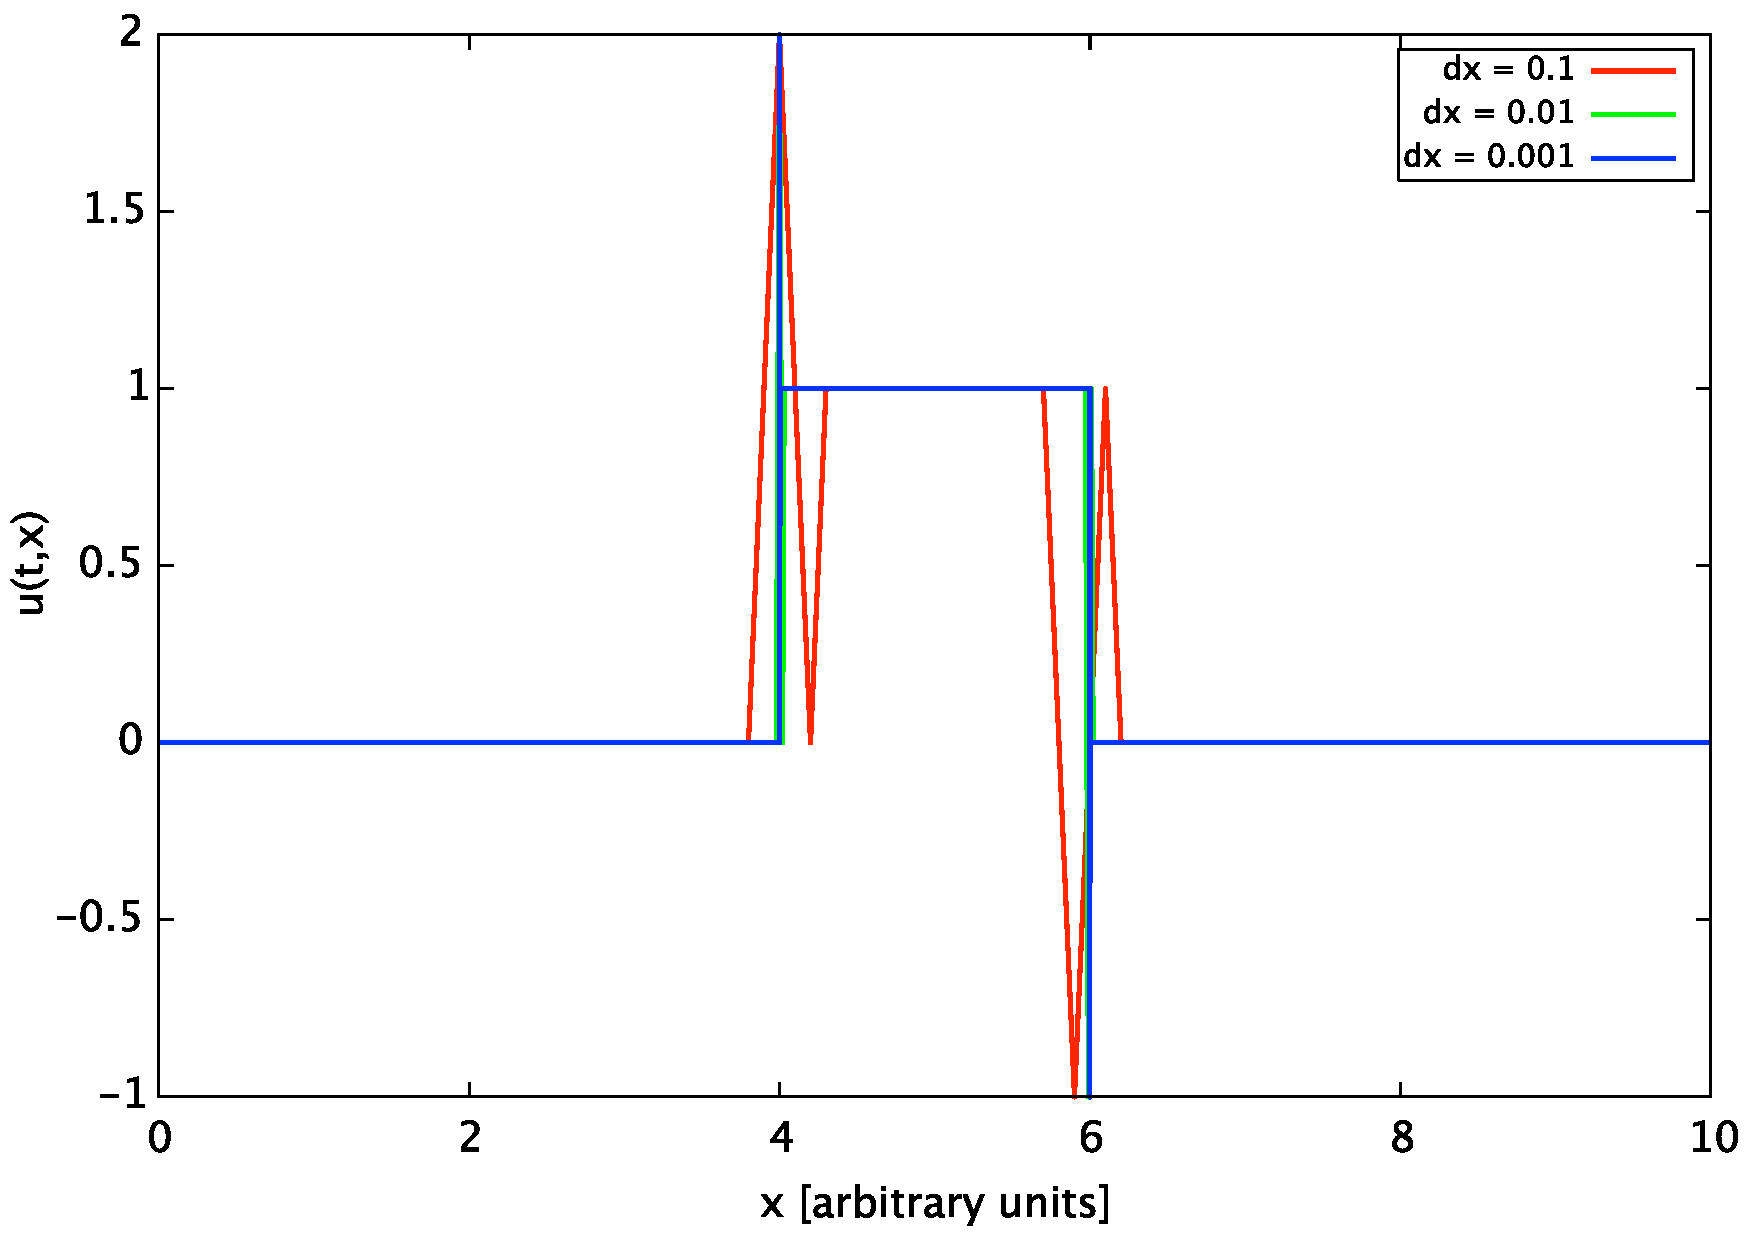
\includegraphics[scale=0.25]{good_img/lf_cf1_t20_s}}
\end{figure}
Therefore, the Leapfrog algorithm with $\Delta x \leq 0.01$ and gaussian initial condition is a reliable method to solve the advection equation, while with square wave initial condition it is not. This fact is underlined by analizing the L2-norm of the algorithm: [da fare]

\section{The Lax-Friedrichs method}
The Lax-Friedrichs method is a stable method (under the condition $|a|\frac{\Delta t}{\Delta x} \leq 1$) to solve the advection equation described by the following algorithm:
\begin{equation}
u_j^{n+1} = \frac{1}{2} (u_{j-1}^n + u_{j+1}^n) - a\frac{\Delta t}{2\Delta x}(u_{j+1}^n - u_{j-1}^n)
\end{equation}
\begin{figure}[!h]
\centering
\subfigure[$u(x,t=10)$ with $c_f=0.5$]
{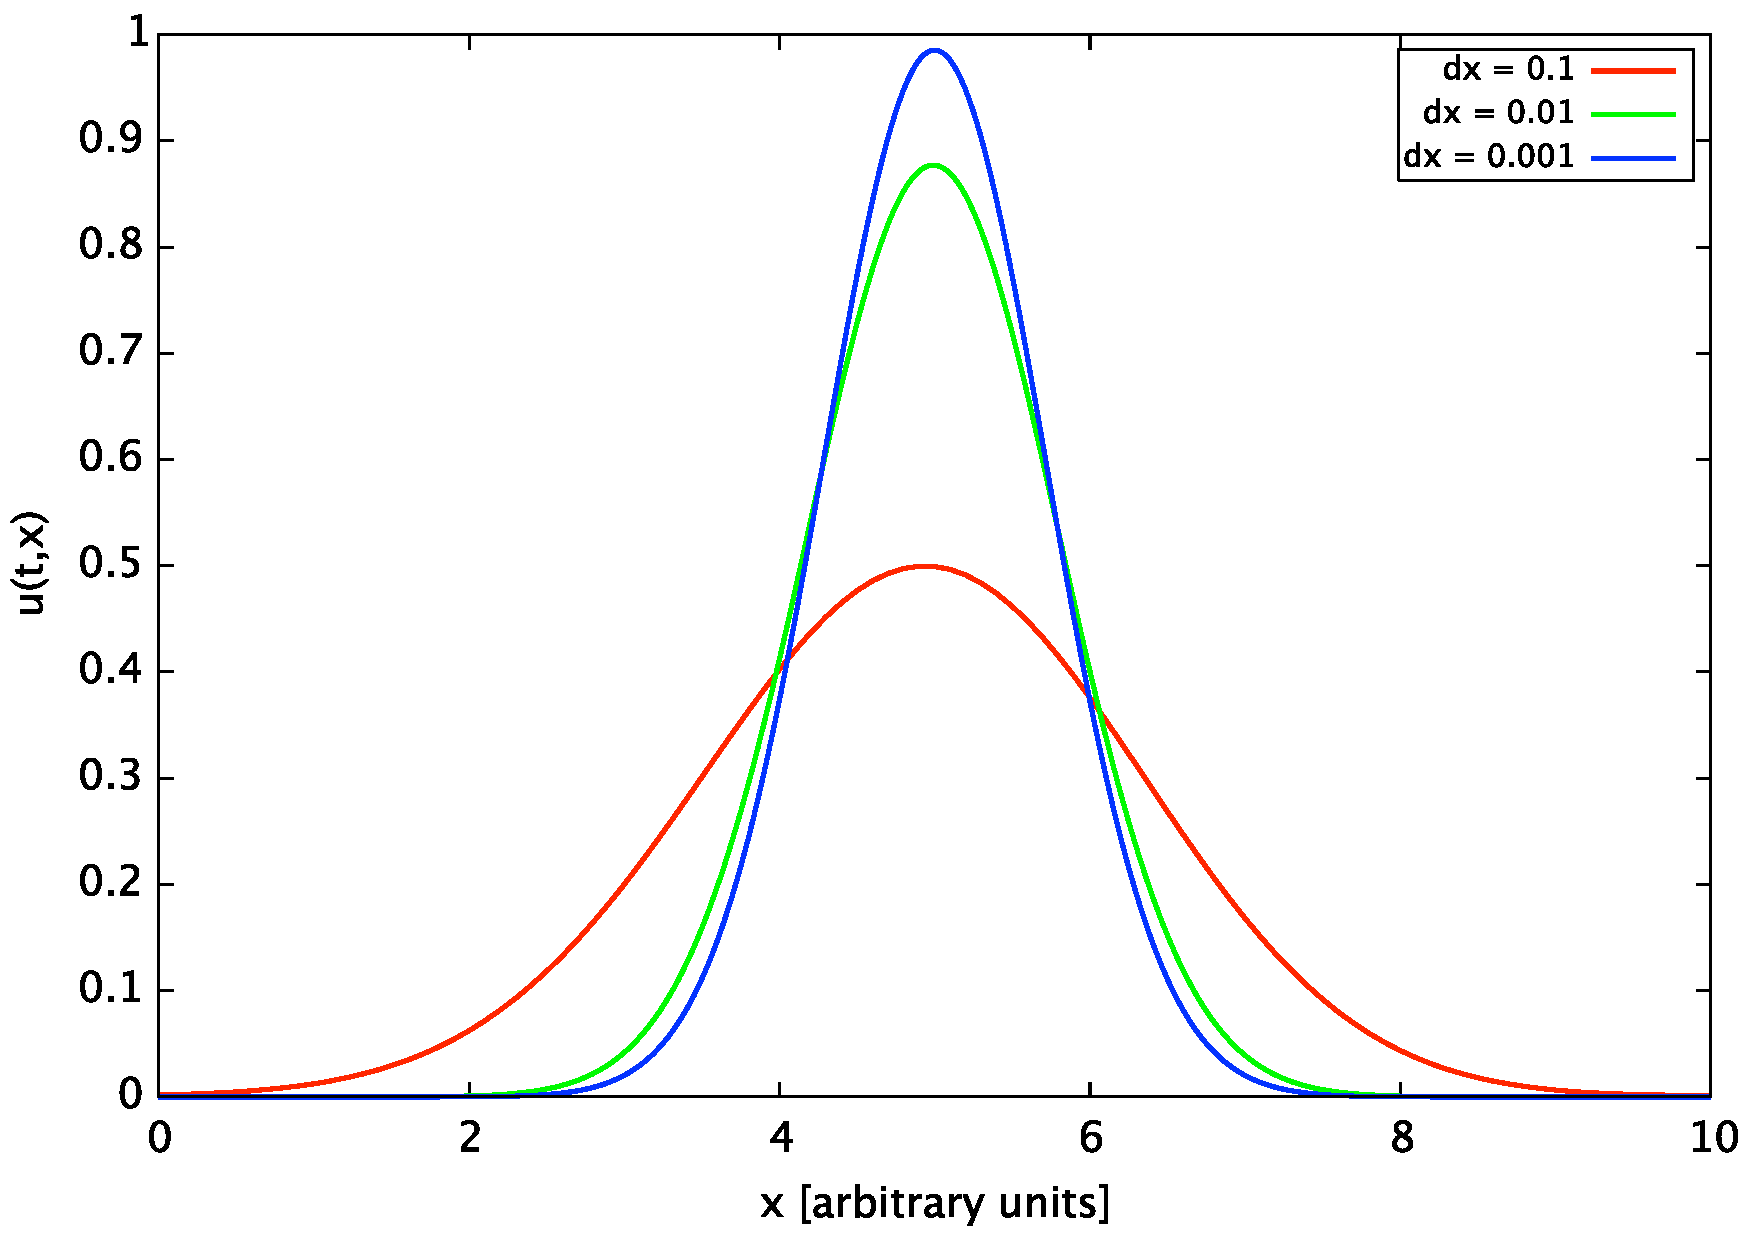
\includegraphics[scale=0.25]{good_img/lxfr_cf05_t10_g}}
\subfigure[$u(x,t=20)$ with $c_f=0.5$]
{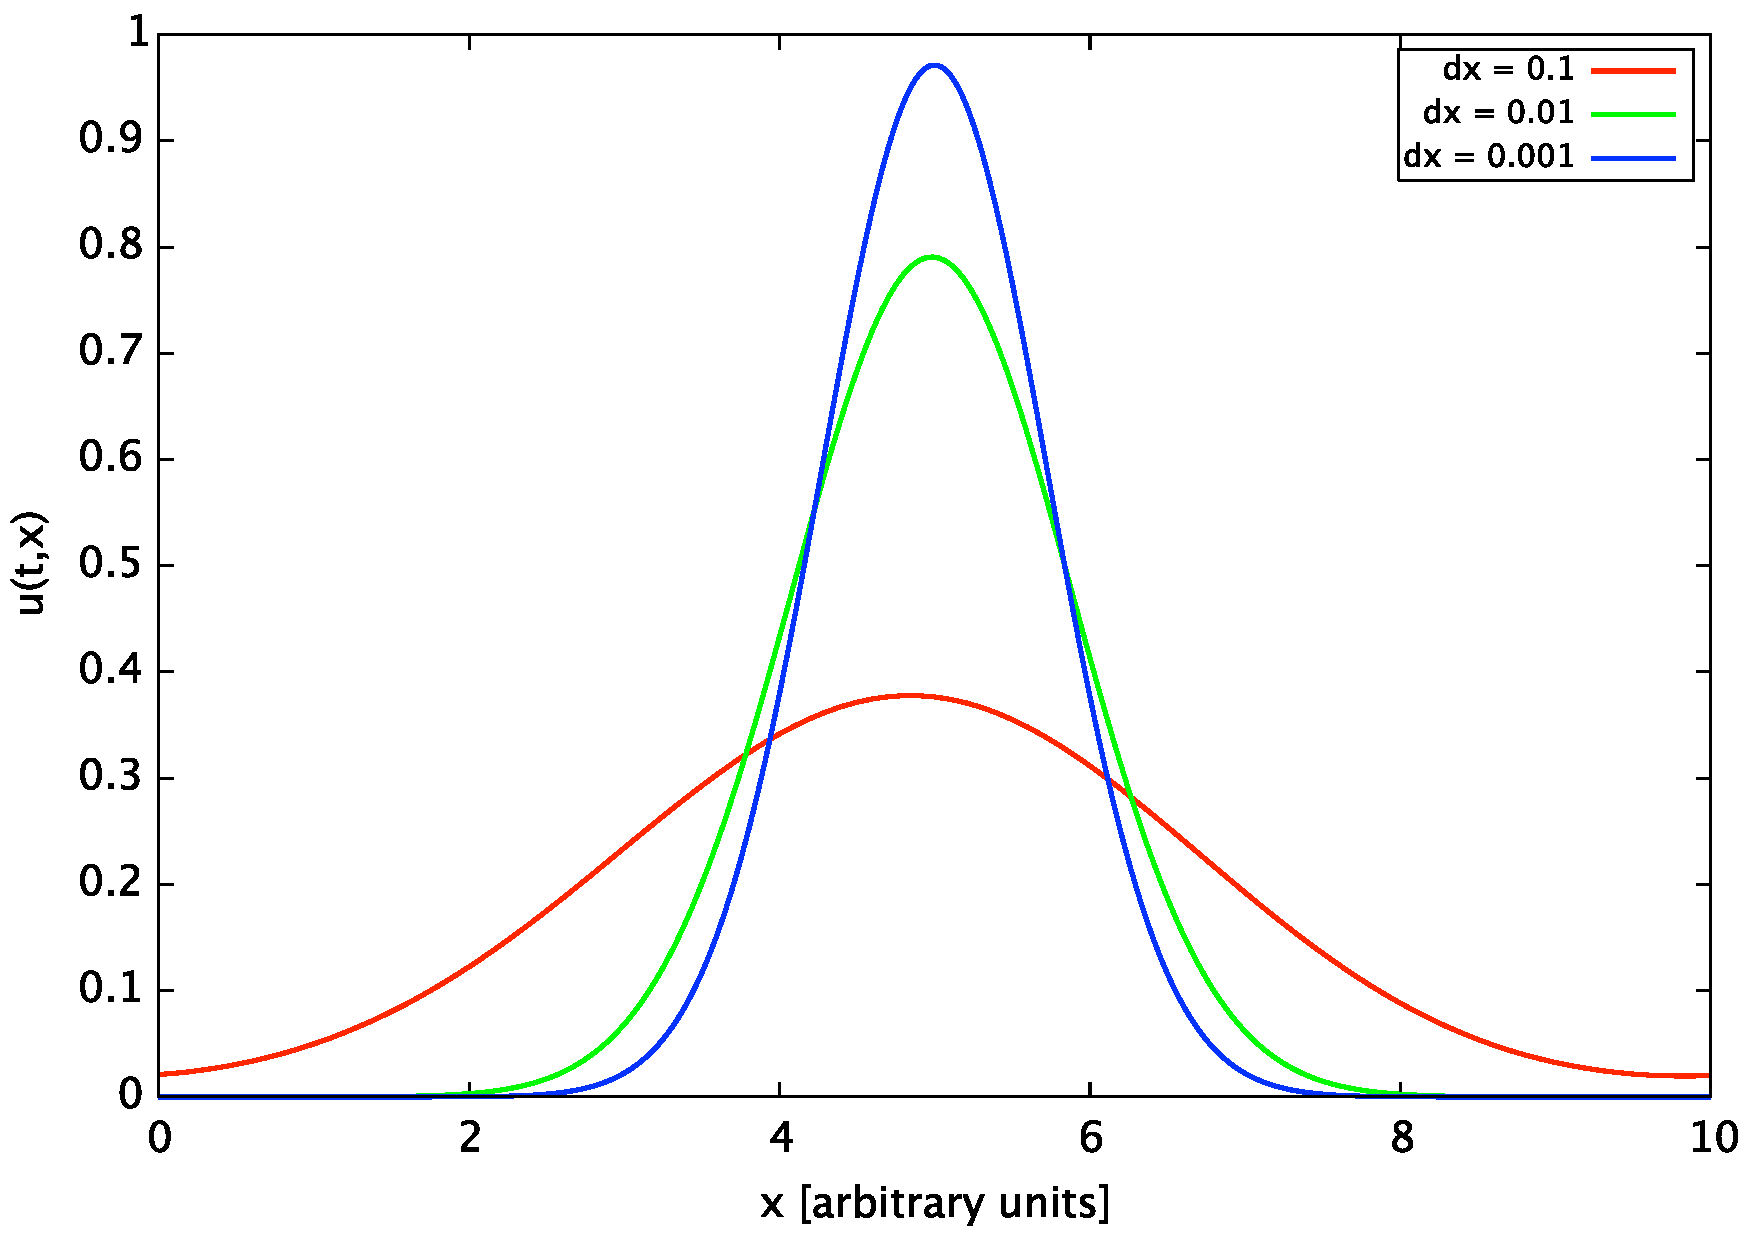
\includegraphics[scale=0.25]{good_img/lxfr_cf05_t20_g}}
\subfigure[$u(x,t=10)$ with $c_f=1$]
{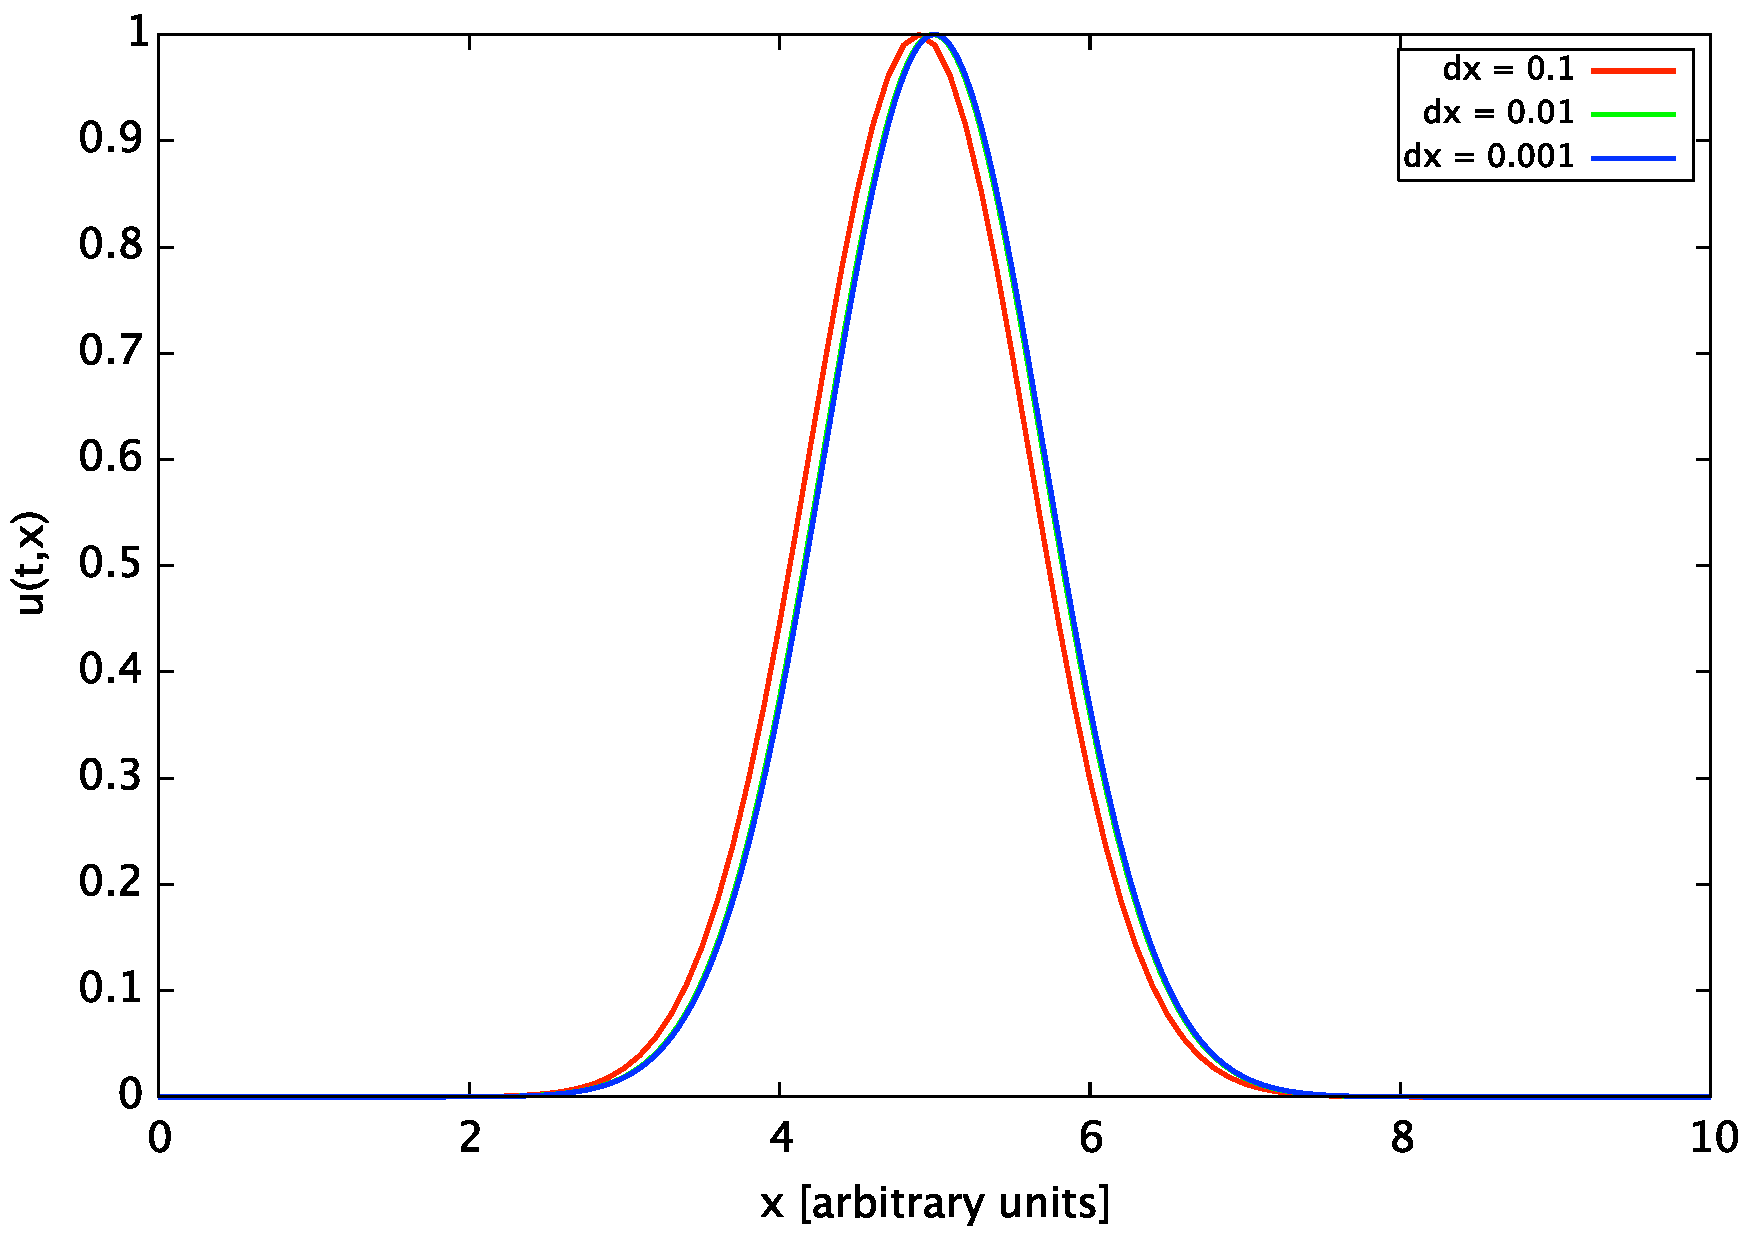
\includegraphics[scale=0.25]{good_img/lxfr_cf1_t10_g}}
\subfigure[$u(x,t=20)$ with $c_f=1$]
{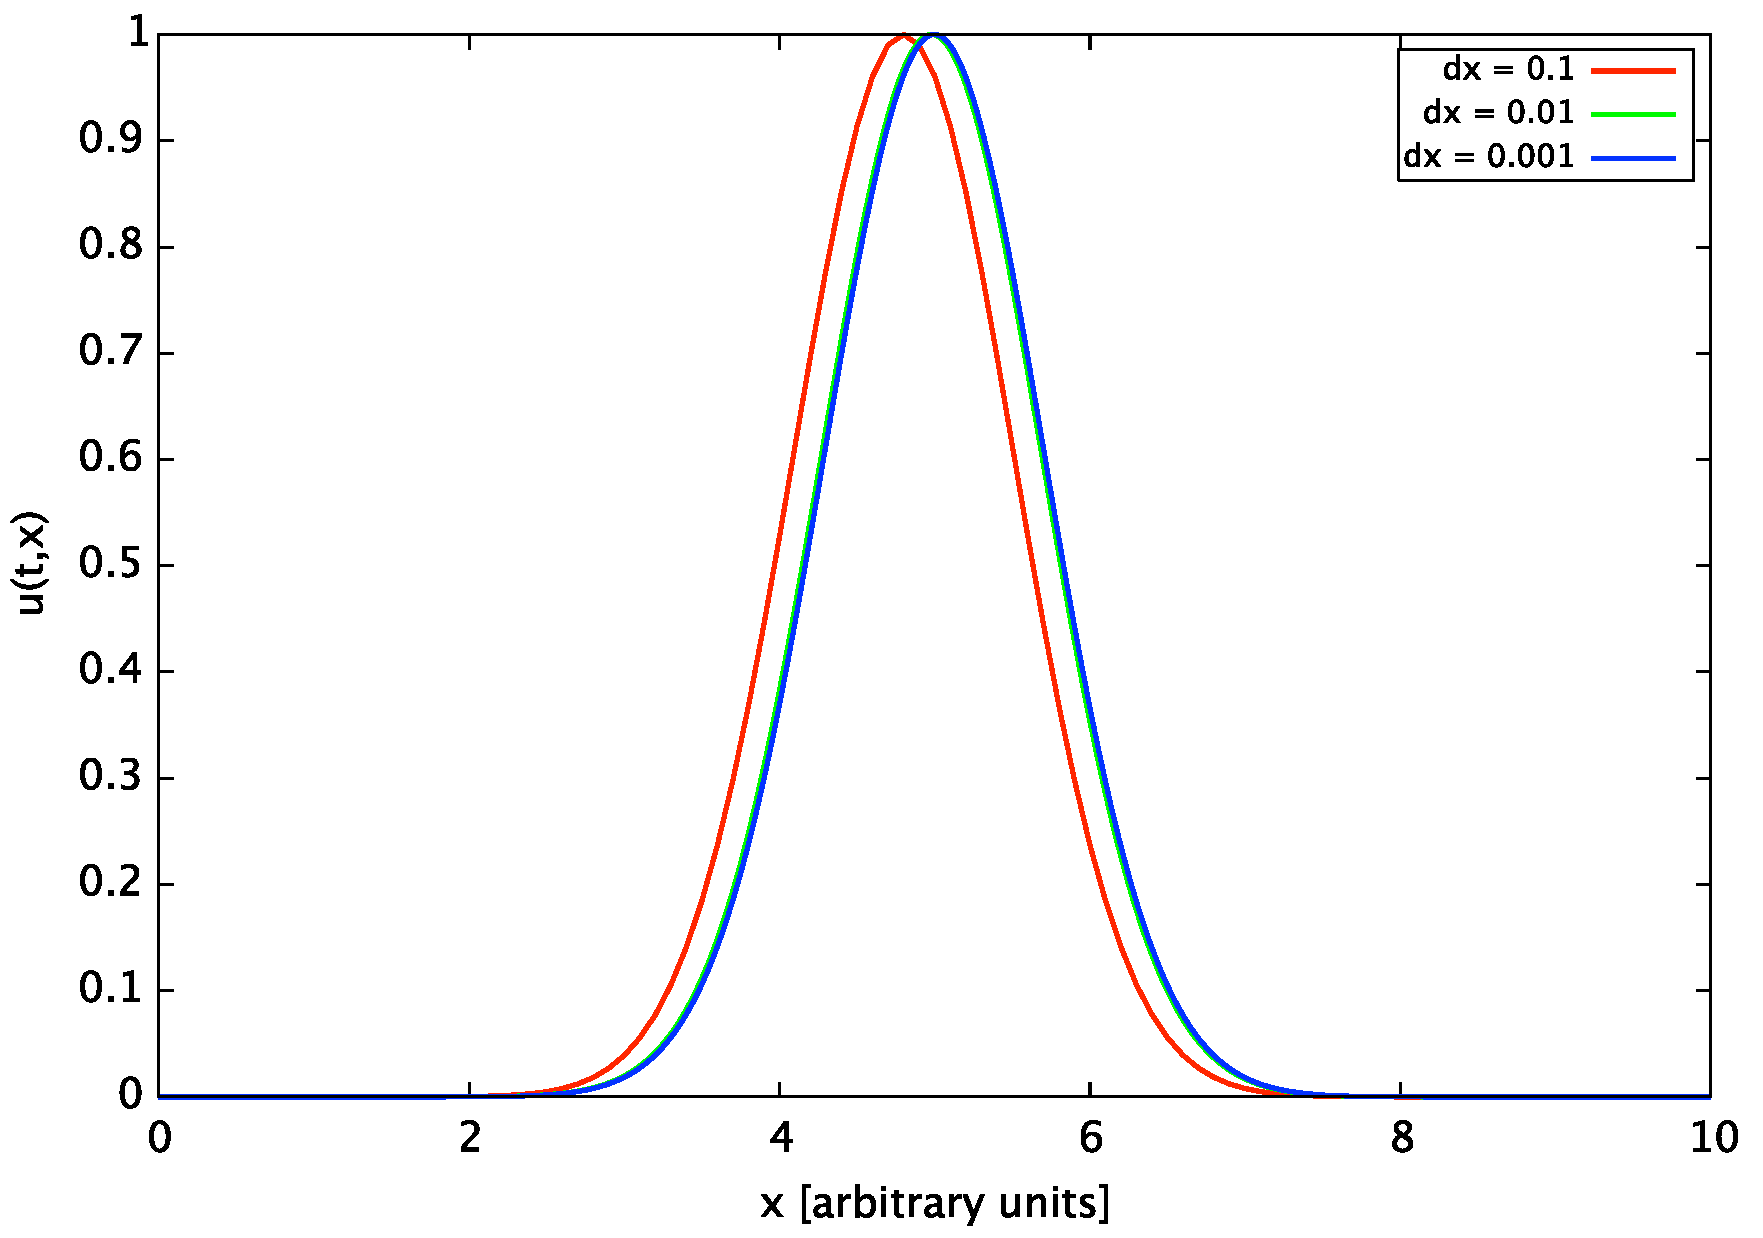
\includegraphics[scale=0.25]{good_img/lxfr_cf1_t20_g}}
\end{figure}\\
where the first factor on the right-hand side of (9) is obtained by substituting $u_j^n$ with its mean value. Let's look at some results obtained implementing the algorithm in different conditions (Fig. (q), (r), (s), (t)). 

\end{document}